\chapter{Phoneme inventories and syllable structure complexity}\label{sec:4}

  The central research questions of this book seek to (i) establish whether highly complex syllable structure is associated with other phonological features such that it can be identified as a coherent linguistic type, and (ii) use these findings to inform diachronic paths of development for these structures. The purpose of this chapter and the ones that follow is to address these research questions by examining other phonological properties of the language sample as they relate to syllable structure complexity. In this chapter I examine the properties of segment inventories in the language sample. Specifically, I test several hypotheses relating the size and constituency of vowel, and especially consonant, inventories to syllable structure complexity.

  The chapter is organized as follows. In \sectref{sec:4.1} I discuss previous findings in the literature regarding properties of consonant and vowel inventories, and accounts put forth to explain predominant crosslinguistic trends in the patterns observed. I then discuss relevant findings relating the structure of sound inventories to syllable structure complexity, and introduce the hypotheses to be tested in the current study. In \sectref{sec:4.2} I describe the methodology behind the data collection and the coding process. In \sectref{sec:4.3} I present a brief analysis of vowel inventory properties and test the hypothesis that syllable structure complexity is associated with larger vocalic nucleus inventories. \sectref{sec:4.4} is a longer section presenting several different analyses testing hypotheses regarding the size and makeup of consonant inventories with respect to syllable structure complexity. In \sectref{sec:4.5} I discuss the results as they relate to highly complex syllable structure, its development, and syllable structure-based phonological typologies more generally.

\section{Introduction}\label{sec:4.1}

  The scope of the current study is limited to examining the properties of segmental phonemes, the more or less discrete units corresponding to contrastive sounds in a language. Suprasegmental properties, including stress and tone, will be considered in \chapref{sec:5}. Certain kinds of variation in segments, including vowel reduction and specific kinds of consonant allophony, will be considered in Chapters~\ref{sec:6} and~\ref{sec:7}.

  A segmental phoneme is an abstract unit corresponding to a set of sounds, usually phonetically similar to one another, which have some functional, cognitive, and/or perceptual equivalence in a language. A language’s phoneme inventory is the group of such units which meaningfully contrast with one another in that language, e.g. /l/ and /b/ in the \ili{English} pair \textit{leek} and \textit{beak}. This concept is well over a century old and has been modified over the years (e.g. \citealt{Sapir1925,ChomskyHalle1968}), but is still widely used in both theoretical models and language descriptions. 

  A disadvantage of phonemic analysis is that it forces a discrete linear analysis on the continuous speech stream. The result of this segmental analysis, some argue, is a theoretical representation which is more reflective of the alphabetic scripts used by many linguists in everyday life than it is of any real property of spoken language (\citealt{Port2006},  \citealt{MorenoCabrera2008}). Noting these problems, some models posit that phonological structures are emergent from more general speech processes. For example, in the Articulatory Phonology framework (\citealt{BrowmanGoldstein1992b}), syllable patterns emerge from the coordination and phasing of gestures. In \citegen{Lindblom2000} model, segments and gestures themselves are adaptations to biophysical constraints on perception and production, as well as cognitive processes of memory encoding. Indeed, alternative views such as Articulatory Phonology and exemplar models of language \citep{Bybee2001} may provide more satisfactory accounts for the fine-grained and gradient nature of sound variation and change. Nevertheless, for all the problematic aspects of phonemic analysis, segment inventories are useful points of comparison in typological studies like the current work. Most language references provide such an analysis at the very minimum, even if no other phonetic or phonological description is given.

  Phoneme inventories are perhaps the best-researched topic in phonological typology, with numerous large-scale surveys dedicated to their study. Standard works on the typology of phoneme inventories occur as early as the mid-20th century (e.g. \citealt{Hockett1955}). The Stanford Phonology Archive \citep{CrothersEtAl1979}, a project undertaken in connection to the Stanford Universals Project, was the first computerized database of phoneme inventories. \citet{Maddieson1984} drew upon this work in his survey of 317 genealogically balanced languages, the UCLA Phonological Segment Inventory Database (UPSID). Since then, many such large typological surveys of phoneme inventories have been developed, including an expanded version of UPSID (451 languages, \citealt{MaddiesonPrecoda1992}), the Lyon-Albuquerque Phonological Systems Database (LAPSyD, {\textasciitilde}700 languages, \citealt{MaddiesonEtAl2013}), PHOIBLE (1,672 languages, \citealt{MoranEtAl2014}), and portions of the World Atlas of Language Structures (WALS, {\textasciitilde}565 languages, \citealt{Maddieson2013b,Maddieson2013c}, inter alia). In addition to these, there have been extensive surveys of phoneme inventories in specific geographical areas (e.g. \citealt{MichaelEtAl2015} for South America, \citealt{GasserBowern2014} for Australia). There are also a great many crosslinguistic studies examining the properties and patterns of specific kinds of sounds, including nasalized vowels \citep{Hajek2013}, non-modal vowels \citep{Gordon1998}, ejectives \citep{Fallon2002}, consonants with secondary palatalization \citep{Hall2000}, affricates \citep{Berns2013}, and post-velar consonants (\citealt{Sylak-Glassman2014}). 

\subsection{Crosslinguistic patterns in consonant inventories}\label{sec:4.1.1}

  In articulatory terms, consonants and vowels are distinguished from one another by the degree to which the vocal tract is constricted in their production, with consonants having greater constriction than vowels. Consonants are typically classified by their articulatory characteristics which include phonation, the place of constriction in the vocal tract, and the manner of constriction.

  Consonant phoneme inventory size is a common point of comparison in cross\-linguistic studies of phonological systems. In the 563-language sample in \citet{Maddieson2013b}, the languages have an average of 22.7 consonant phonemes,\linebreak though values range widely from six consonants (in \ili{Rotokas}) to 122 consonants (in !Xóõ). There are areal patterns to the distribution of consonant inventory size. Small inventories (6--14 consonants) are common in New Guinea and the Amazon region of South America. Large consonant inventories (26 or more consonants) are concentrated in the Pacific Northwest and northern coast of North America, northern Europe, the Caucasus region, and regions of  Africa.

  One of the contributions of the 317-language survey in \citet{Maddieson1984} was the establishment of crosslinguistic frequency patterns for consonant phonemes. The following consonants are the 20 most frequently present in the inventories of the language sample (* indicates that dental and alveolar consonants have been pooled).

\ea\label{ex:4.1}
  /p b *t *d k ɡ ʔ t͡ʃ f *s ʃ h m *n ɲ ŋ w *l *r j/
\citep[12]{Maddieson1984}
\z

None of the consonants in \REF{ex:4.1} were found to occur in every language in the sample, and some (/ʔ t͡ʃ f ʃ ɲ r/) were found in fewer than half of the languages. It follows that strict implicational hierarchies derived from these frequency measures do not accurately predict the makeup of observed consonant phoneme inventories, small or large. Nevertheless, all spoken languages have at least several of these consonants, even though there are hundreds of other consonants from which inventories could hypothetically be entirely drawn. The constituency of this set of consonants in terms of numbers of stops, fricatives, nasals, and so on closely resembles the modal makeup of consonant inventories in the sample overall. \citet{LindblomMaddieson1988} note that this set of consonants is nearly identical to that reported for stages of early speech and babbling. Furthermore, in a sample of 32 diverse languages, \citet[73--74]{Gordon2016} finds that there is a strong positive correlation between the frequency of these consonants crosslinguistically (that is, across consonant inventories) and the type frequency of these consonants within languages.

  The convergence of these patterns suggests a phonetic naturalness to the consonants in \REF{ex:4.1} which many researchers have attempted to account for. \citet{Stevens1989} shows that there are configurations of articulators within the vocal tract where the acoustic and auditory properties of the sound produced there are fairly stable with respect to variations in the articulation. He suggests that these regions of acoustic-perceptual stability underly the common distinctions found in phoneme inventories. \citet{Maddieson1996} proposes that phonological patterns are motivated by gestural economy, in that optimal contrastive sounds will involve gestures which are both inherently efficient in their motor requirements and have a high degree of auditory distinctiveness. Other accounts take a more abstract approach. \citet{Ohala1979} observes that consonants in small phoneme inventories may be perceptually close to one another and differ by a minimum rather than maximum of distinctive features. On the basis of this he proposes that consonant phoneme inventories are motivated by a principle of \textit{Maximum Utilization of Available Features} (MUAF). In a similar vein, \citet{Clements2003} proposes that consonant inventories tend towards economy in their constituency; that is, sounds are less likely to occur in a language if their distinctive features are not employed elsewhere in the phoneme inventory, and more likely to occur if all their distinctive features occur elsewhere in the phoneme inventory. The set of consonants in \REF{ex:4.1} is quite coherent in this respect. A typological study of borrowed sounds lends support to these accounts: \citet{Maddieson1985} finds that borrowed sounds are statistically much more likely to fill gaps in the phonological inventory of the recipient language than to alter the basic contrasts of the system.

  \citet{LindblomMaddieson1988} propose an account for the observed crosslinguistic tendencies which is rooted in properties of articulatory complexity. In their model, consonants are divided into three sets: Set I, basic articulations which often correspond to those in \REF{ex:4.1}; Set II, elaborated articulations corresponding to properties described below; and Set III, complex articulations, consisting of combinations of elaborated articulations. Elaborated articulations are defined as those which depart from default modes of phonation and manner (especially airstream mechanism), as well as place articulations which depart from the neutral near-rest positions of active articulators in the vocal tract. A list of these elaborations is reproduced in \tabref{tab:4.1}.

\begin{table}
\begin{tabularx}{\textwidth}{lQQ}
\lsptoprule
{Phonation} & {Manner} & {Place}\\\midrule
breathy voice                  & prenasalization  &labiodental\\
creaky voice                   & nasal release    &palatoalveolar\\
voiced fricatives/affricates   & lateral release  &retroflex\\
voiceless sonorants            & ejectives        &uvular\\
pre-aspiration                 & implosives       &pharyngeal\\
post-aspiration                & clicks           &palatalization\newline labialization\newline pharyngealization\newline velarization\\
\lspbottomrule
\end{tabularx}
\caption{\label{tab:4.1}Elaborated consonant articulations, as presented in \citet[67]{LindblomMaddieson1988}.}
\end{table}

The model predicts that as consonant inventory sizes increase, languages will include phonemes from Set I (e.g. /k/) until that set is more or less exhausted, at which point Set II consonants (e.g. /kʷ/) and then eventually Set III consonants (e.g. /kʷ’/) may occur. Lindblom \& Maddieson show that this prediction is borne out in the obstruent inventories of the 317-language sample from \citet{Maddieson1984}. They suggest that these patterns, at all levels of consonant inventory size, reflect a balance between competing pressures to keep articulatory complexity low while maintaining a sufficient level of perceptual contrast in the system \citep[72]{LindblomMaddieson1988}.

  There are of course many other issues related to consonant inventory patterns which are too numerous to discuss here (e.g. common gaps in stop inventories with respect to place of articulation and voicing). An overview of many such patterns and proposed phonetic accounts for them can be found in \citet{Ohala1983}.

  The issues of consonant phoneme inventory size and elaborated articulations will be revisited in \sectref{sec:4.1.3} and \sectref{sec:4.1.4}. In the following section I discuss reported typological patterns of vowel phoneme inventories.

\subsection{Crosslinguistic patterns in vowel inventories}\label{sec:4.1.2}

  As described above, vowels are speech articulations which involve relatively less constriction in the vocal tract than consonants. Vowels are typically classified according to the height and backness of the tongue body and the rounding of the lips, which together constitute vowel ``quality''. Other articulatory characteristics, such as length, nasalization, and voicing may also be contrastive for these sounds, but only in addition to vowel quality.

 \hspace*{-0.19002pt}Perhaps the most common point of typological comparison for vowel phoneme systems is the number and nature of vowel qualities present. Over half of the languages in the 564-language survey in \citet{Maddieson2013c} have five or six vowel qualities present in their phoneme inventories. Like consonant phoneme inventory size, vowel quality inventory size has strong areal patterns with respect to its distribution. Smaller than average systems are common in the Americas, Australia, and isolated smaller regions. Larger than average systems are common in the central belt region of Africa, Southeast Asia, and parts of Eurasia. Areal patterning may also be observed in other vowel features, including contrastive nasalization, which is predominantly concentrated in Western Africa and the Amazon region.

  The five most common vowel quality phonemes in \citegen{Maddieson1984} survey are /i a u “o” “e”/ (where quotations indicate that these may not be distinguishable from other vowels in the mid area in the references consulted). Unlike the situation with consonants above, there are many languages which have a triangular system of five vowels corresponding exactly to this set (1984: 136). Generally speaking, there are strong crosslinguistic tendencies relating the size of vowel quality inventories to the vowel qualities observed to occur. For example: for example, three-vowel systems are most often of the shape /i a u/. 

  As with crosslinguistic tendencies in consonant inventories, both acoustic/perceptual and articulatory accounts have been put forward to explain the observed patterns in vowel quality inventories. \citet{LiljencrantsLindblom1972} test the hypothesis that vowel inventories pattern in such a way as to maximize perceptual distance, measured as a function of formant values. The predictions of their model match very closely the most common vowel quality inventories for vowel systems of three, four, and five vowels, but for larger inventories, there are discrepancies between the model and observed crosslinguistic patterns. The study by \citet{Stevens1989} mentioned above considered vowel systems in addition to consonant systems, and determined /i a u/ to be regions of acoustic/perceptual stability with respect to articulatory variation. \citet{LindblomMaddieson1988} also explored vowel inventory patterns and concluded that as with consonant systems, common vowel system patterns reflect competing pressures of maximization of perceptual contrast and minimization of articulatory complexity. Thus it is not expected that articulatorily ``complex'' contrasts such as those involving phonation, nasalization, length, and so on would be present in a system of five total vowels, where perceptual distinctiveness can be easily achieved by vowel quality differences alone. Analogous to their model of consonant elaborations, differences in phonation, nasalization, and so on should be expected to occur only in larger systems where vowel quality contrasts have already been exploited. From a diachronic point of view, such contrasts in vowel systems typically imply larger vowel inventories because they come about through sound changes that are systematic across the vowel system or large portions of the vowel system.

\subsection{Segmental inventories and syllable structure complexity}\label{sec:4.1.3}

  The crosslinguistic patterns described above and the proposed accounts for them are limited to phoneme inventories themselves and do not consider possible interactions between phoneme inventories and other aspects of language structure. Yet a number of correlations between phoneme inventories and other phonological structures, most notably syllable structure complexity, have been found.

  \citet{Maddieson2006} determined that there is a highly significant positive correlation between consonant phoneme inventory size and syllable structure complexity in a sample of roughly 520 languages. In that study, it was found that languages with Simple syllable structure had an average of 19.3, languages with Moderately Complex syllable structure an average of 21.8, and languages with Complex syllable structure an average of 25.7 consonant phonemes (\citealt{Maddieson2013a} reports similar findings). Within that sample, there are some overlapping geographical distributions of small consonant inventories and simpler syllable structures on the one hand and large consonant inventories and more complex syllable structure on the other hand. The Pacific Northwest region of North America is an example of a region with the latter pattern, and the Amazon Basin is an example of a region with the former pattern. However, Maddieson rejects the idea that the overall correlation was the result of several small-scale patterns, finding the general trend to hold up significantly in all but one of the large geographical regions examined. He concludes that the association between consonant phoneme inventory size and syllable structure complexity is crosslinguistically robust and suggests that “paths of natural historical linguistic change” may be behind this mutually reinforcing pattern of complexity (2006: 118). 

  Consonant phoneme inventory size is positively correlated with syllable structure complexity when it is measured in non-categorical ways, too. \citet{Maddieson2011} reports a positive correlation between consonant inventory size and Syllable Index values. The Syllable Index is a sum of maximal onset, nucleus, and coda complexity values, closely but not perfectly corresponding to the number of segments in the maximal syllable type. \citet{Gordon2016} plots consonant inventory size against the sum of maximal syllable margins for each language in the modified WALS 100-language sample and finds an increasing, if not stepwise trend. He reports similar results for analyses considering only onset or coda size.

  There has been limited research into the patterns of specific segment types and syllable structure complexity. \citet{MaddiesonEtAl2013} report a relationship between segmental complexity in phoneme inventories and syllable structure complexity in the {\textasciitilde}700-language LAPSyD sample. In that study they consider the number of consonants with one or more elaborated articulations, as defined by \citet{LindblomMaddieson1988} and listed in \tabref{tab:4.1} above. They find that languages with Complex syllable structure have a mean of 9.6 consonants with elaborated articulations, as compared to means of 6.2 and 4.8 such consonants in the Moderately Complex and Simple categories, respectively. The difference between the Complex pattern and the two other patterns combined was found to be statistically significant.

  There have also been suggestions of correlations between phoneme inventory properties and other phonological features at smaller scales, within regions or language families. In his holistic phonological typology of Slavic languages, \citet{Isačenko1939/1940} notes that ``consonantal'' languages are defined by a collection of features, including more complex syllable structure, a larger proportion of consonants in the phoneme inventory, and the presence of contrastive secondary palatalization at various places of articulation. \ili{Russian} and \ili{Polish} are prototypical examples of such languages. By comparison, ``vocalic'' languages have simpler syllable structure, smaller proportions of consonants in the phoneme inventory, and secondary palatalization which is limited to dental consonants or altogether absent. The Ljubljana dialect of \ili{Slovene} exemplifies this type. \citet[43]{Chirikba2008} calls all languages of the Caucasus “consonant-type languages”, a term which encompasses a heavy dominance of consonants over vowels in the speech signal, rich consonant inventories, and restricted vowel systems. Chirikba specifically notes the typologically unusual nature of consonant systems in the languages of the region, which include ejectives and richly elaborated sibilant and post-velar articulations.

  The above observations bring up another relationship worth mentioning,\linebreak which is that between consonant inventory size and vowel inventory size. While no correlation has ever been established between consonant inventory size and \textit{vowel quality} inventory size \citep{Maddieson2013c}, a positive correlation has been found between consonant inventory size and \textit{total vowel} inventory size \citep{Maddieson2011}. In that study, the ``total vowel inventory'' includes vowels which contrast in length, nasalization, and phonation properties, as well as diphthongs analyzed as unitary, but does not include tautosyllabic vowel sequences or diphthongs that can be parsed into constituents corresponding to basic vowels in the language.

\subsection{The current study and hypotheses}\label{sec:4.1.4}

  The findings described above indicate that the relationship between properties of segment, and especially consonant, inventories and syllable structure complexity is notable at global, regional, and family levels, and thus worthy of further investigation. The hypotheses I introduce and test here build on the previous findings by investigating the relationships between more specific properties of phoneme inventories and syllable structure complexity. Depending on their nature, these findings may help to shed light on those paths of language change suggested by \citet{Maddieson2006} to motivate the observed correlations.

  The first hypothesis concerns vocalic nucleus inventory size and syllable structure complexity. Recall that in \sectref{sec:3.3.4} it was found that complex vocalic nuclei, defined there as long vowels, diphthongs, and/or tautosyllabic vowel sequences, were more frequently present in languages with more complex syllable structure. There is reason to explore this pattern in more depth here. As noted above, a positive correlation between total vowel inventory size and consonant phoneme inventory size has been established in the literature \citep{Maddieson2011}. However, the measure of total vowel inventory size did not include tautosyllabic vowel sequences or diphthongs that can be alternatively analyzed as sequences of segments. Thus it would be interesting to test whether a relationship exists between the \textit{total number of vocalic nuclei} in a language and syllable structure complexity. If such a relationship is found, it would suggest that higher syllable margin diversity is accompanied by higher nucleic diversity in languages with more complex syllable structure, a fact that would have to be considered in any diachronic account of the development of highly complex syllable structure. The hypothesis is formulated in \REF{ex:4.2}.

\ea\label{ex:4.2}
  As syllable structure complexity increases, languages will have larger inventories of vocalic nuclei.
\z

  This is the only hypothesis regarding vowel patterns in the sample. The remaining hypotheses are concerned with consonant patterns. The second hypothesis follows the findings of \citet{Maddieson2006}, and simply predicts that the previously determined positive association between syllable structure complexity and consonant phoneme inventory size will be upheld when the additional category of Highly Complex syllable structure is included in the analysis. Following observations by \citet{Gordon2016}, I also expect that consonant phoneme inventory size will increase with syllable structure complexity when it is measured not just categorically but also as a sum of maximal syllable margins. This hypothesis is given in \REF{ex:4.3}.

\ea\label{ex:4.3}
  As syllable structure complexity increases, so does the size of consonant phoneme inventories.
\z

  The third hypothesis is aimed at quantifying the number of articulatory elaborations present in the consonant inventories of languages with different syllable structure complexity. \citet{MaddiesonEtAl2013} found a higher mean number of consonants with elaborated articulations in languages with more complex syllable structure. However, the reported findings of that study did not consider whether languages with more complex syllable structure also had more distinct elaborations present in their consonant inventories. That is, the findings do not indicate whether languages with more complex syllable structure have more elaborations in general, or just more consonants sharing the same elaboration. Reported phonological patterns for areas well-known for having complex syllable patterns suggest the presence of more elaborations in their consonant inventories (e.g. ejectives and uvulars in the Caucasus, lateral release and ejectives in the Pacific Northwest). This would also follow indirectly from \citet{LindblomMaddieson1988}, who found consonants with combinations of elaborated articulations in languages with large consonant inventories. This leads to the formulation of a third hypothesis, given in \REF{ex:4.4}.

\ea\label{ex:4.4}
  As syllable structure complexity increases, so does the number of articulatory elaborations present in consonant phoneme inventories.
\z

  The final hypothesis relates syllable structure complexity to the occurrence of specific consonant types. This hypothesis is motivated by the observation that there are certain consonants which seem characteristic of languages with more complex syllable structure. Specifically, post-velar and especially uvular consonants, though crosslinguistically rare, are common in regions also famous for complex syllable structure, including the Pacific Northwest, the Caucasus, and the Atlas Mountain region. Similarly, it is my observation that ejectives are often found in languages with complex syllable structure, and often co-occur with uvular consonants in those languages. Based on these observations, a fourth hypothesis is formulated.

\ea\label{ex:4.5}
  Languages with differing degrees of syllable structure complexity will exhibit different consonant contrasts in their phoneme inventories.
\z

  The data analyses addressing these hypotheses will be presented in \sectref{sec:4.3} and \sectref{sec:4.4}. In the next section I describe the methodology behind the data collection and coding for these analyses.

\section{Methodology}\label{sec:4.2}
\subsection{Patterns considered}\label{sec:4.2.1}

  In this chapter, only the segmental patterns of the language sample are considered. While most of the analyses here will treat specific articulations that do not constitute segments on their own (i.e. those associated with place, manner, voicing, length, etc.), it must take as a starting point the consonant and vowel phoneme inventories of the language sample. These are understood to be the more or less discrete units which are mostly unpredictable in their distribution and meaningfully contrastive in the native lexicon and grammar of a language. Though consonant and vowel phoneme inventories are reliably reported in most language references, phonemic analysis is not always a straightforward endeavor. Here I discuss some issues that arise in determining phoneme inventory patterns.

  Phonemic inventories are always the result of an analysis. It is common for there to be slight disagreements regarding the composition of the phoneme inventory in different descriptive materials for the same language. Authors may be writing in different time periods, describing different dialects and/or speech styles, or, in the case of highly endangered languages, working with speakers with varying degrees of proficiency in the language. When sources disagree on just a few elements of the phoneme inventory, I take these factors into consideration. For example, two of the sources on \ili{Nuu-chah-nulth}, \citet{Stonham1999} and \citet{Davidson2002}, list uvular ejectives /q’ qʷ’/ in the consonant phoneme inventory, but a third source \citep{Kim2003} does not. The former analyses are based primarily on the field notes of Edward Sapir, who worked with the language from 1914--1924. \citet{Kim2003} shows that ejective uvulars have long since merged with pharyngeal /ʕ/ in the present language. I take the more recent analysis to be accurate for the current state of the language. 

  Of course, the choices made in a phonemic analysis may reflect a number of other factors, including the data available and the author’s own theoretical training and native language biases. When sources present dramatically different phoneme inventories, I accept the source which supports the analysis more thoroughly with illustrative language-internal data. For example, \citet{CunhadeOliveira2005} presents a consonant phoneme inventory for \ili{Apinayé} which includes an entire prenasalized consonant series which is not listed in \citet{BurgessHam1968}, who take a more abstract approach. Cunha de Oliveira shows that although prenasalized consonants are often in complementary distribution with nasals in the language, there are minimal pairs showing that these sounds are meaningfully contrastive in some environments, an observation that is reinforced by reported native speaker intuition about the forms.

  Sounds which are limited to recent loanwords, the speech of bilinguals, and certain speech styles were not included in the present study. For instance, in \ili{Cocopa}, mid front vowel /e/ is described as occurring only in loanwords from \ili{Spanish} and \ili{English}, and even then is often replaced by native /i/ \citep[26]{Crawford1966}. In \ili{Tzeltal}, voiceless labial fricative /f/ and alveolar trill /r/ are reported to occur only in loanwords in the speech of ``acculturated'' \ili{Spanish} bilinguals \citep[13]{Kaufman1971}. In \ili{Chipaya}, glottal stop /ʔ/ occurs in one obsolescing morpheme, \textit{-ʔa}, a declarative suffix formerly used by women to address other women (\citealt{Cerrón-Palomino2006}: 55--56). In all these and similar cases, the given sounds were omitted from the current analysis.

  Authors of language descriptions often present marginal phonemes -- those occurring with very low frequency, highly limited distributions, or in just a few lexical items -- in addition to more straightforward ones. Where authors show these to be contrastive in lexical items, I have generally included such phonemes here. Where a marginal phoneme is described as clearly obsolescing or merging with another sound to the point that the contrast is no longer meaningful for most speakers of the variety examined, I have excluded it.

  As mentioned in \sectref{sec:3.2.1}, sounds with multiple articulations, such as labialized consonants, affricates, or diphthongs, present obvious complications for a study of this sort. The analysis of a phonetic sequence, such as [mb], as either a sequence of two simple segments or as a single complex segment can in turn affect how the canonical syllable patterns of a language are analyzed.\footnote{{Of course, these issues may not prove so problematic in an Articulatory Phonology framework, or any model which does not force a discrete segmental analysis upon sound and syllable patterns.}} Because issues such as these may create a potential confound in how we interpret associations between syllable structure complexity and segmental inventories, it is important that competing analyses be carefully evaluated. 

  Instrumental data can be used to support either a complex segment analysis or a sequential analysis in such a scenario. For example, if a phonetic sequence of homorganic nasal+stop has a durational pattern comparable to that of a simple voiceless stop in a language, this might be taken as evidence for a complex segment analysis (e.g. as shown for \ili{Fijian} by \citealt{Maddieson1989a}; though \citealt{LadefogedMaddieson1996} note that there is wide crosslinguistic variation in timing patterns in prenasalized consonants). There are a few studies on such issues in languages of the current sample. For example, \citet{Chitoran1998} uses acoustic evidence to argue that \ili{Georgian} harmonic clusters (e.g. [dɡ], [tʰkʰ]) are better analyzed as sequences than as complex segments, as some have claimed. She shows that each member of a harmonic cluster has a release burst, and that the durational properties of these clusters word-internally do not differ significantly from identical sequences found across word boundaries. However, it is generally very rare in the language descriptions consulted here for authors to present acoustic or articulatory evidence supporting one analysis over another in such situations. In the absence of instrumental data, authors often rely on phonological criteria to support their analyses.

  Sometimes authors base their analyses on distributional data. \citet[135--138]{Erickson2001} argues that phonetic C+[w] structures in \ili{Lao} are in fact labialized consonants and not onset clusters. He observes that no corresponding C+[j] sequences (or palatalized consonants, for that matter) occur as onsets in the language, and that C+[w] structures are infrequent and limited in their distribution, occurring almost entirely before the low vowel /ɑ/ and never before rounded vowels. These facts suggest a historical process by which the consonant in C+[u] sequences may have taken on the rounding of the high back vowel, a crosslinguistically common type of assimilation. Note that in this case, either analysis puts the language in the Moderately Complex category in the current study.

  Similar criteria are used to posit a series of prenasalized consonants in \ili{Tukang Besi}. If these structures were considered to be sequences, then they would be the only consonant clusters occurring in the language, which otherwise has canonical (C)V structure. Prenasalized consonants behave as a unit in reduplication processes; that is, words like \textit{karambau} have \textit{kara-karambau} as a reduplicated form, instead of \textit{karam-karambau}. (This argument assumes a syllabification of \textit{ka.ram.bau} in the scenario that [mb] is a sequence and not a complex segment). Additionally, native speakers put syllable breaks before the nasal+C sequences when dividing words into syllables \citep[30--31]{Donohue1999}. 

  The \ili{Tukang Besi} evidence is not strictly conclusive. The language could be analyzed as having (C)(C)V syllable structure which has very specific restrictions on C\textsubscript{2} and C\textsubscript{1}. In this case the ambiguous interpretation has important consequences for syllable structure complexity: one interpretation puts the language into the Simple category, while the other puts it into the Complex category. There is just one language in the Complex category, \ili{Lunda}, which has biconsonantal onset patterns fitting the hypothetical (C)(C)V pattern for \ili{Tukang Besi}. However, in \ili{Lunda} other biconsonantal onsets, like C+glide sequences, also occur, and the nasal+C sequences may come about through morphological processes (that is, some are morphologically separable; example 6).

\ea\label{ex:4.6}
\etriple{Lunda}{Atlantic-Congo}{Democratic Republic of Congo, Angola, Zambia}

/ku-n-ʒikwila/

\textsc{inf}-\textsc{1.sg}-uncover

[ku.nʒi.kwi.la]\\
\glt ‘to uncover for me’
\citep[24]{Kawasha2003}
\z

In \ili{Lunda} onsets, nasals may combine with a wide variety of consonants, including all plosives, oral fricatives, /h/, /l/, and /w/. In \ili{Tukang Besi}, the C in nasal+C structures is always an oral plosive or /s/, though other fricatives and sonorants occur in the language. There is persuasive evidence that nasal+C structures are sequences in \ili{Lunda}. The nasal+C structures in \ili{Tukang Besi} do not have much in common with those of \ili{Lunda} in terms of their behavior. Though the evidence for the unitary status of prenasalized consonants in \ili{Tukang Besi} is not entirely conclusive, I follow the author’s analysis here, coding these structures as complex segments and classifying the language as having Simple syllable structure. 

  A similar issue arises in interpreting a phonetic sequence of a mid or low vowel followed by a high offset. This can be analyzed as a diphthong, in which case the entire structure functions as a syllable nucleus, or a sequence of V+glide, in which case the glide is a member of the coda. Competing analyses for such structures can be found in \ili{Yakima Sahaptin}. Structures represented orthographically as <ay>, <aw> <uy>, and so on, are described as diphthongs by \citet{Jansen2010} and \citet{RigsbyRude1996}. However, \citet{HargusBeavert2006} present evidence that the structures ending in the high front articulation may be better analyzed as V+/j/ sequences. Preceding /m/, these structures trigger a vowel epenthesis process that is also conditioned by other sonorant consonants, but not vowels, in the language \REF{ex:4.7}.\pagebreak

\ea\label{ex:4.7}
  \etriple{Yakima Sahaptin}{Sahaptian}{USA}

\ea /t͡ɬ’jálm/\\\relax
  [t͡ɬ’jálɨm]
\glt  ‘Cle Elum (place name)’

\ex  /talújm/\\\relax
  [talújɨm]
\glt   ‘nail’

\ex  /naknúwim/\\\relax
  [naknúwim]
\glt  ‘take care of me’ \citep[28]{HargusBeavert2006}
\z
\z

This is presented as evidence that the high front element in these structures behaves as a consonant. Though the /w/ component of such sequences is not reported to trigger the epenthesis process in \REF{ex:4.7}, it is reported to pattern with /j/ in other morphophonemic contexts, and \citet{HargusBeavert2006} treat it as a consonant in their analysis. This analysis has the effect of increasing the maximal coda pattern of the language to four, in which all four-consonant codas begin with a glide, e.g. \textit{sajlps} ‘kidney’. However, due to other syllable patterns in the language, it does not affect the syllable structure complexity classification, which in either case is Highly Complex.

  \ili{Kunjen} presents an example of a language for which a sequential analysis rather than a complex segment analysis results in patterns which directly affect its syllable structure complexity classification. \citet[34]{Sommer1969}  rejects a prenasalized stop analysis for structures such as [mb] and [ŋɡ] on the basis that reverse sequences occur and all component segments may occur separately. This analysis is what allows \ili{Kunjen} to be classified as having Highly Complex syllable structure in the current study, as nasal+stop sequences are always present in the four-consonant codas in the language, which are also the only Highly Complex structures occurring \REF{ex:4.8}.

\ea\label{ex:4.8}
   \etriple{Kunjen}{Pama-Nyungan}{Australia}

/albmb/\\
\glt ‘opossum’
\citep[33]{Sommer1969}
\z

  It should be noted that it was generally rare for ambiguous segmental analyses to affect the analysis of syllable structure to the point where a language might be classified in a different syllable structure complexity category. In fact the \ili{Tukang Besi} and \ili{Kunjen} examples discussed here are the most potentially problematic cases in the entire language sample.

\subsection{Coding}\label{sec:4.2.2}

  After the above criteria were considered and segmental inventories determined, properties of the vowel and consonant inventories were coded as described here.

  Vowel inventories were coded for all reported contrasts. First, the number of vowel quality distinctions was noted. Every vowel inventory was additionally coded for the presence or absence of contrastive vowel length, nasalization, and other less common contrasts, such as voicing and glottalization. Where such contrasts were present, it was noted whether the contrast was distinctive for all or some vowels. 

  I also noted the presence of diphthongs and/or tautosyllabic vowel sequences and recorded the number and specific forms of these structures. Because they are so often analyzed as phonological sequences which surface phonetically as diphthongs, diphthongs present complications in establishing vowel phoneme inventory patterns \citep[133]{Maddieson1984}. Recall that the purpose of considering patterns of diphthongs and tautosyllabic vowel sequences here is to establish the size of the full vocalic nucleus inventory for each language in order to test the hypothesis in \REF{ex:4.2}. Therefore the diphthongs and tautosyllabic vowel sequences included in the inventories are not necessarily meant to be interpreted as phonologically unitary segments, but as possible nucleus patterns if reported as occurring as such.

  In \REF{ex:4.9} I illustrate the coding with the vowel phoneme inventory of \ili{Pinotepa Mixtec}, a language with Simple syllable structure.

\ea\label{ex:4.9}
\etriple{Pinotepa Mixtec}{Otomanguean}{Mexico}
\begin{Coding}
\item[V phoneme inventory:] /i e a o u ĩ  ẽ  ã  õ  ũ  ḭ  ḛ  a̰  o̰  ṵ ḭ ḛ  a̰  o̰  ṵ/
\item[\textit{N} vowel qualities:] 5
\item[Diphthongs or vowel sequences:] None
\item[Contrastive length:] None
\item[Contrastive nasalization:] All
\item[Other contrasts:] Glottalization (All)
\end{Coding}
\z

  For each consonant inventory, the number of non-geminate consonants was recorded. Each consonant inventory was first coded for primary distinctions in voicing, place, and manner of articulation; here I use the term ``primary'' to refer to those distinctions represented in the standard chart for non-pulmonic consonants in the International Phonetic Alphabet \citep{IPA2015}.\footnote{{Note that I use different terminology than IPA in some cases: ``stop'' instead of ``plosive'', and ``palato-alveolar'' instead of ``postalveolar''.}} The presence of a primary voiced/voiceless distinction was noted separately for obstruents and sonorants; voicing had to be the sole distinguishing feature for at least one pair of consonants in order for this distinction to be counted (e.g. /k/ and /ɡ/, /m̥/ and /m/). All primary manners of articulation in the inventory were recorded, as were the primary places of articulation for all non-glide consonants. Additionally, I recorded the presence of elaborated articulations related to phonation, manner, and place, as defined by \citet{LindblomMaddieson1988} and listed in \tabref{tab:4.1} above. Note that there is some overlap in what I take to be primary articulations and the articulations classified as elaborations by Lindblom \& Maddieson (e.g. labiodental, uvular); in the coding such articulations are included in both the place/manner lists and in the list of elaborations.

  In \REF{ex:4.10} I illustrate the coding with the consonant phoneme inventory of \ili{Lepcha}, a language with Complex syllable structure.

\ea\label{ex:4.10}
  \etriple{Lepcha}{Sino-Tibetan}{Bhutan, India, Nepal}
\begin{Coding}
\item[C phoneme inventory:] 
\item[] /p pʰ b t̪ t̪ʰ d̪ ʈ ʈʰ ɖ c cʰ k kʰ ɡ ʔ t͡s t͡sʰ f v s z ʃ ʒ h m n̪ ɲ ŋ r l̪ β ̞ j/

\item[\textit{N} consonant phonemes:] 32

\item[Geminates:] N/A

\item[Voicing contrasts:] Obstruents

\item[Places:] Bilabial, Labiodental, Dental, Alveolar, Palato-alveolar, Retroflex, Palatal, Velar, Glottal

\item[Manners:] Stop, Affricate, Fricative, Nasal, Trill, Central approximant, Lateral approximant

\item[\textit{N} elaborations:] 5

\item[Elaborations:] Voiced fricatives/affricates, Post-aspiration, Labiodental, Palato-alveolar, Retroflex
\end{Coding}
\z

Dental and alveolar places of articulation are not always reliably distinguished in reference materials \citep[31--32]{Maddieson1984}. Sometimes authors even use the joint label ``dental/alveolar'' as a cover term for a series of consonants in that general area in the vocal tract. In such cases, I characterize the place of the consonants in question as Dental/Alveolar \REF{ex:4.11}.

\ea\label{ex:4.11}
  \etriple{Southern Grebo}{Atlantic-Congo}{Liberia}
\begin{Coding}
\item[C phoneme inventory:] \item[] /p b t d c ɟ k ɡ k͡p ɡ͡b f s h m̥ m n̥ n ɲ ŋ ŋ͡m l̥ l w̥ w j/
\item[Places:] Labial-velar, Bilabial, Dental/Alveolar, Palatal, Velar, Glottal
\end{Coding}
\z

  The current study considers only non-geminate consonant phonemes. Geminates are not always given the same treatment as consonants of normal length in phonological descriptions, as they often occur in specific morphological contexts. While there are languages in which consonant gemination is contrastive within morphemes, there are many more in which gemination is contrastive at the lexical level but only in morphologically complex contexts. As a result of this, discussions of gemination are often presented in the context of morphophonological processes, and comprehensive lists of geminate consonants may not be given and sometimes must be inferred. As the hypotheses in this chapter are concerned with phonation, place, and manner articulations, issues of consonant gemination are not considered in any depth. However, the reported presence of gemination in consonant inventories is noted in the coding in Appendix~\ref{sec:Appendix:B}.

  The phoneme inventory coding for each language in the sample, along with other notes on the consonant and vowel systems, can be found in Appendix~\ref{sec:Appendix:B}. In the following sections I present the results of the analyses of consonant and vowel inventories. Because only one of the hypotheses in the current chapter relates to vowel inventories, I present this study first.

\section{Results: Vowel inventories}\label{sec:4.3}

  In this section, I describe vowel inventory patterns in the language sample. The purpose of the study here is twofold: first, to test the hypothesis in \REF{ex:4.2} regarding vocalic nucleus inventory size and syllable structure, and second, to explore general features of vowel contrast with respect to syllable structure complexity. For the latter, there are no explicit hypotheses, but any patterns uncovered will be noted in the event that they might help shed light on the development of syllable structure complexity.

\subsection{Vowel quality inventory size}\label{sec:4.3.1}

  The distribution of vowel quality inventory sizes in the languages of the sample can be found in \figref{fig:4.1}.


\begin{figure}
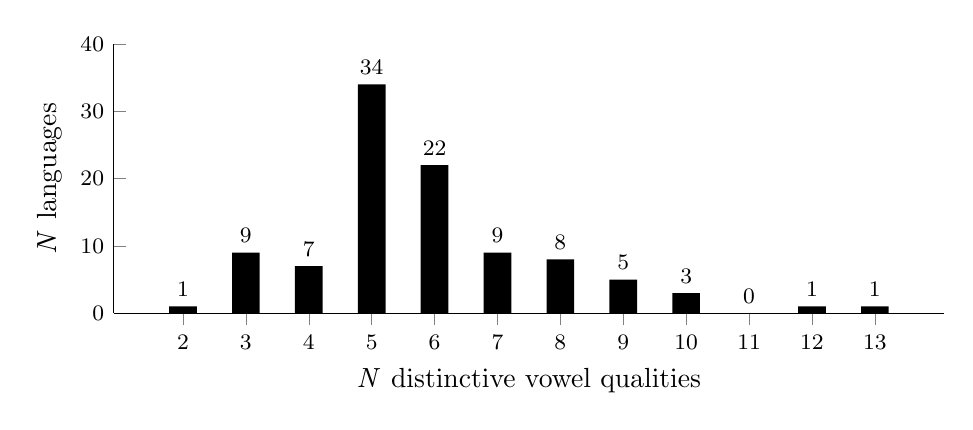
\begin{tikzpicture}
            \begin{axis}[
                    ybar,
                    ylabel={\textit{N} languages},
                    xlabel={\textit{N} distinctive vowel qualities},
                    xtick=data,
                    axis lines*=left,
                    ymin=0,
                    ymax=40,
                    scaled y ticks=false,
                    legend pos=north west,
                    ticklabel style={font=\footnotesize\scshape},
                    width=\textwidth,
                    height=5cm,
                    enlarge x limits={0.1},
                    nodes near coords,
                    nodes near coords style={text=black,font=\footnotesize},
                    ]
                \addplot+[
                     fill=black,draw=none
                    ] table {
                    x   y
                    2	1
3	9
4	7
5	34
6	22
7	9
8	8
9	5
10	3
11	0
12	1
13	1                  
};
\end{axis}
\end{tikzpicture}
\caption{\label{fig:4.1}Languages of sample distributed according to the number of distinctive vowel qualities in their phoneme inventories.}
\end{figure}

  The average number of distinctive vowel qualities for languages in the sample is 5.9. The range is 2--13, with the extremes being \ili{Kabardian} (two vowel qualities) and \ili{Eastern Khanty} (13 vowel qualities). Over one-third (34) of the languages have systems with five contrastive vowel qualities. The next most common pattern is for languages to have six contrastive vowel qualities. These proportions are nearly identical to those reported for the 564-language sample in \citet{Maddieson2013c}.

  The mean, median, and range of vowel quality inventory sizes for the languages in each category of syllable structure complexity can be found in \tabref{tab:4.2}.

\begin{table}
\begin{tabular}{lcccc}
\lsptoprule
 & \multicolumn{4}{c}{Syllable structure complexity}\\\cmidrule(lr){2-5}
\textit{N} vowel qualities & S & MC & C & HC\\
                           & 24 lgs. & 26 lgs.    & 25 lgs. & 25 lgs.\\\midrule
{Mean} & 5.8 & 6.2 & 6.2 & 5.3\\
{Median} & 5 & 6 & 5 & 5\\
{Range} & 4--9 & 3--13 & 4--10 & 2--9\\
\lspbottomrule
\end{tabular}
\caption{\label{tab:4.2}Vowel quality inventory sizes in each syllable structure complexity category.}
\end{table}

  There are no clear trends with respect to mean or median vowel quality inventory size and syllable structure complexity. Statistical analysis shows no significant correlation between vowel quality inventory size and syllable structure complexity, measured either categorically ($r(100) = -0.078$, $p > 0.05$) or as a sum of maximal syllable margin sizes ($r(100) = -0.038$, $p > 0.05$).

\subsection{Contrastive vowel length}\label{sec:4.3.2}

  In this section, I examine patterns of contrastive vowel length in the sample. Here I include all languages reported to have contrastive vowel length for some or all vowel qualities. I also include six languages (\ili{Ewe}, \ili{Fur}, \ili{Kambaata}, \ili{Maori}, \ili{Maybrat}, and \ili{Nimboran}) which are described as having tautosyllabic sequences of identical vowels, and two languages (\ili{Carib} and \ili{Selepet}) which are described as having diphthongs consisting of identical vowels. In the latter groups of languages, other non-identical vowel sequences or diphthongs are typically present, and phonetically long vowels are often found in morphologically complex contexts. Together, these facts are often used by authors to justify a sequential analysis rather than a contrastive vowel length analysis. I include these languages in the current analysis because the structures in question are reported to be produced as phonetically long vowels which may meaningfully contrast with short vowels (\ref{ex:4.12}a--b).

\ea\label{ex:4.12}
\etriple{Maybrat}{Maybrat-Karon}{Indonesia}

\ea  /puut/\\{}
  [puːt]\\
\glt  ‘we climb’

\ex  /put/\\{}
  [put]\\
\glt  ‘leech’
\citep[29]{Dol2007}
\z
\z

  The distribution of contrastive vowel length in the languages of the sample according syllable structure complexity can be found in \tabref{tab:4.3}.

\begin{table}
\begin{tabularx}{\textwidth}{Icccc}
\lsptoprule
 & \multicolumn{4}{c}{Syllable structure complexity}\\\cmidrule(lr){2-5}
Vowel length & S & MC & C & HC\\
             & \textit{N} = 24 & \textit{N} = 26 & \textit{N} = 25 & \textit{N} = 25\\\midrule
{Contrastive} & 8 & 8 & 13 & 11\\
{Tautosyllabic sequences or diphthongs of identical Vs} & 1 & 6 & 1 & --\\
{Non-contrastive} & 16 & 12 & 11 & 14\\
\lspbottomrule
\end{tabularx}
\caption{\label{tab:4.3}Contrastive vowel length in the sample. Note that Maori (in the Simple category) is reported to have contrastive vowel length for one vowel quality, but tautosyllabic sequences of identical vowels for other vowel qualities. (In Maori, nearly all possible combinations of two vowels can be found to occur tautosyllabically in normal speech. \citet[524--528]{Bauer1999} uses this distribution to justify the analysis of all phonetically long vowels as sequences of identical vowels. However, phonetic [aː] has a much higher frequency than would be expected if a sequential analysis were accepted, so Bauer analyzes this particular vowel quality as having contrastive length, while [iː], [ɛː], etc. are taken to be sequences.) Therefore the numbers in the Simple column add up to 25.}
\end{table}

  Over half of the languages in the sample (53/100) do not have contrastive vowel length. Vowel length distinctions are somewhat less common in the languages of the Simple category than those of the other categories; however, this trend is not significant in a chi-square test. In terms of geographic distribution, all six macro-areas examined here have four or more languages with vowel length contrasts, with this pattern being most common in North America (12 languages) and least common in Eurasia (four languages).

  The above analysis does not distinguish between languages which have vowel length contrasts for all vowel qualities and those that have them for only some. In \figref{fig:4.2} below, I present such an analysis, examining only those languages with contrastive vowel length, including those with tautosyllabic sequences or diphthongs of identical vowels.

\begin{figure}
\caption{\label{fig:4.2} Proportion of languages in each syllable structure complexity category which have contrastive vowel length for some or all vowel qualities (VQs).}
\begin{tikzpicture}
\pgfplotstableread{data/fig42.csv}{\table}
    \pgfplotstablegetcolsof{\table}
    \pgfmathtruncatemacro\numberofcols{\pgfplotsretval-1}
            \begin{axis}[easterdaystacked,cycle list={{Greys-F},{Greys-K}},
                                xticklabels={S,MC,C,HC},
                        ]
            \foreach \i in {1,...,\numberofcols} {
                \addplot+[
                    /pgf/number format/read comma as period, fill
                    ] table [x index={1},y index={\i},x expr=\coordindex] {\table};
                \pgfplotstablegetcolumnnamebyindex{\i}\of{\table}\to{\colname} % Adding column headers to legend
                \addlegendentryexpanded{\colname}
            }
            \end{axis}                                                                           
\end{tikzpicture}
\end{figure}

  In all categories, languages with vowel length contrasts are generally more likely to have these contrasts for all rather than just some vowel qualities. However, there is an interesting result with respect to vowel length contrasts in the Simple syllable structure category. Although languages with Simple syllable structure are overall less likely to have vowel length contrasts, if they do have a contrast they are also most likely to have this contrast for all vowel qualities. In fact, this pattern is without exception in the language sample.

  Below I illustrate the prominent patterns in vowel length distinctions with the vowel inventories of two languages: \ili{Rotokas}, which has Simple syllable structure and length contrasts for all qualities, and \ili{Dizin}, which has Complex syllable structure but length contrasts only for a subset of vowels \xxref{ex:4.13}{ex:4.14}.

\ea\label{ex:4.13}
  \etriple{Rotokas}{North Bougainville}{Papua New Guinea}
   \begin{Coding}
\item[V phoneme inventory:] /i e a o u iː eː aː oː uː/
   \end{Coding}
\z

\ea\label{ex:4.14}
  \etriple{Dizin}{Dizoid}{Ethiopia}
\begin{Coding}
\item[V phoneme inventory:] /i e ɛ ɨ ɑ o u iː eː ɑː oː uː/
   \end{Coding}
\z

\subsection{Other vowel contrasts}\label{sec:4.3.3}

  Here I present analyses of other contrastive properties present in the vowel inventories of the language sample, namely nasalization and phonation contrasts. See \tabref{tab:4.4} for the distribution of languages in the sample with respect to contrastive vowel nasalization.

\begin{table}
\begin{tabular}{lcccc}
\lsptoprule
 & \multicolumn{4}{c}{Syllable structure complexity.}\\\cmidrule(lr){2-5}
Vowel nasalization & S & MC & C & HC\\
             & \textit{N} = 24 & \textit{N} = 26 & \textit{N} = 25 & \textit{N} = 25\\\midrule
{Contrastive} & 9 & 4 & 4 & 4\\
{Non-contrastive} & 15 & 22 & 21 & 21\\
\lspbottomrule
\end{tabular}
\caption{\label{tab:4.4}Vowel nasalization contrasts in the sample}
\end{table}

  Roughly one-fifth of the languages (21/100) have a vowel nasalization contrast for some or all vowel qualities. This feature is much more common in languages with Simple syllable structure, occurring in over a third of languages in that category, as compared to a much smaller proportion of languages in the other categories; this trend is statistically significant in Fisher’s exact test ($p = 0.04$). Contrastive vowel nasalization is also strongly associated with particular geographic regions in the current sample: all but four of the languages with this feature are found in Africa, North America, and South America. This distribution closely mirrors the areal patterns noted by \citet{Hajek2013} in a 244-language sample. As compared to the analysis of vowel length contrasts in \sectref{sec:4.3.2}, there is no clear pattern in the sample with respect to the presence of nasalization contrasts for some or all vowel qualities and syllable structure complexity.

  We now turn to an analysis of phonation contrasts in the vowel inventory data. These are not common, but do occur in six languages in the sample, listed in \tabref{tab:4.5} by the specific kind of phonation contrast and syllable structure complexity.

\begin{table}
\begin{tabularx}{\textwidth}{IQQQI}
\lsptoprule
 & \multicolumn{4}{c}{Syllable structure complexity}\\\cmidrule(lr){2-5}
\hangindent=0pt {Other vowel contrasts} & {Simple} & {Moderately Complex} & {Complex} &\hangindent=0pt {Highly Complex}\\\midrule
Contrastive voicing & \textit{Ute} & \textit{(\ili{Kambaata})} & \textit{--} & \textit{Tohono O’odham}\\
Contrastive glottalization/creaky voice & {\textit{Pinotepa\newline\hspace*{.5em}Mixtec}}\newline\textit{Sichuan Yi} & \textit{Pacoh} & \textit{Mamaindê} & \textit{--}\\
\lspbottomrule
\end{tabularx}
\caption{\label{tab:4.5}Languages in sample with distinctive phonation contrasts in vowel inventories, according to syllable structure complexity. The phonological status of voiceless vowels in Kambaata is not fully determined: it is not entirely predictable, but neither is it contrastive in the traditional sense (that is, participating in clear minimal pairs, \citealt[20--22]{Treis2008}).}
\end{table}

  In this very small data set, contrastive phonation in vowel inventories is more likely to be found in languages with Simple or Moderately Complex syllable structure. Nearly every language with a phonation contrast in its vowel inventory also has an additional contrast besides vowel quality: either vowel nasalization (two languages) or vowel length (four languages). The only exception to this trend is \ili{Sichuan Yi}. I illustrate these patterns with the vowel phoneme inventories of \ili{Ute} and \ili{Mamaindê} \xxref{ex:4.15}{ex:4.16}.

\ea\label{ex:4.15}
  \etriple{Ute}{Uto-Aztecan}{USA}
\begin{Coding}
\item[V phoneme inventory:] /i œ a ɯ u iː œː aː ɯː uː i̥ œ̥ ḁ ɯ̥ u̥/
\end{Coding}
\z

\ea\label{ex:4.16}
  \etriple{Mamaindê}{Nambiquaran}{Brazil}
\begin{Coding}
\item[V phoneme inventory:] /i e a o u ĩ  ẽ  ã  õ  ũ  ḭ ḛ a̰ o̰ ṵ ı̰̃  \~{ḛ} ã̰  õ̰  ṵ̃/
\end{Coding}
\z

\subsection{Diphthongs and vowel sequences}\label{sec:4.3.4}

  In this section I analyze other vocalic nucleus patterns in the sample, specifically patterns of diphthongs and tautosyllabic vowel sequences. This analysis excludes the diphthongs or vowel sequences made up of identical vowels that were included in the analysis of contrastive vowel length in \sectref{sec:4.3.2}. I group together diphthongs and vowel sequences here because the terms are often used interchangeably to refer to the same or very similar tautosyllabic structures, sometimes even within the same language reference. See \tabref{tab:4.6} for the distribution of languages according to syllable structure complexity and the presence or absence of diphthongs or vowel sequences.

\begin{table}
\begin{tabularx}{\textwidth}{Qcccc}
\lsptoprule
 & \multicolumn{4}{c}{Syllable structure complexity}\\\cmidrule(lr){2-5}
Diphthongs or vowel sequences & S & MC & C & HC\\
     & \textit{N} = 24 & \textit{N} = 26 & \textit{N} = 25 & \textit{N} = 25\\\midrule
{Present} & 8 & 14 & 8 & 8\\
{Absent} & 16 & 12 & 17 & 17\\
\lspbottomrule
\end{tabularx}
\caption{\label{tab:4.6}Languages of the sample, distributed according to syllable structure complexity and the presence or absence of diphthongs or tautosyllabic vowel sequences.}
\end{table}

  Languages with Moderately Complex syllable structure are much more likely than languages from the other categories to have diphthongs or vowel sequences (just over half of the languages in this category have these patterns, as compared to roughly one-third of the languages in the other categories).

  There is a very wide range in the size of diphthong and tautosyllabic vowel sequence inventories in the languages of the sample. Extremely large inventories of diphthongs or vowel sequences, as illustrated by the 23-diphthong system of \ili{Selepet}, are rare \REF{ex:4.17}. \ili{Selepet} has six vowel qualities, and nearly all possible combinations of vowels are reported to occur, either as diphthongs or sequences of identical vowels (which were included in the analyses in \sectref{sec:4.3.2}). The modal value for the 38 languages in the sample with diphthongs or tautosyllabic vowel sequences is just two such structures, as illustrated for \ili{Telugu} \REF{ex:4.18}.

\ea\label{ex:4.17}
\etriple{Selepet}{Nuclear Trans New Guinea}{Papua New Guinea}
\begin{Coding}
\item[Diphthongs:] \item[] /ie ia iɔ io iu ei eu ai ae ao au ɔi ɔe ɔo ɔu oi oe ou ui ue ua uɔ uo/
\end{Coding}
\z

\ea\label{ex:4.18}
\etriple{Telugu}{Dravidian}{India}
\begin{Coding}
\item[Diphthongs:] /ai au/
\end{Coding}
\z

\subsection{Vocalic nucleus inventories and syllable structure complexity}\label{sec:4.3.5}

  Here I combine the results of the above analyses in order to determine whether there is any positive correlation between the size of vocalic nucleus inventories and syllable structure complexity, as hypothesized in \sectref{sec:4.1.4}.

  This hypothesis was motivated by observations in \sectref{sec:3.3.4}, where it was found that greater syllable structure complexity was associated with a higher likelihood of a language having complex vocalic nuclei, defined there as long vowels, diphthongs, and/or tautosyllabic vowel sequences. It was assumed that the stronger presence of complex vocalic nuclei might correspond to overall larger vocalic nucleus inventories in languages with more complex syllable structure, revealing a relationship between vowel inventories and syllable structure complexity which has not been previously reported. However, the results in §§\ref{sec:4.3.2}--\ref{sec:4.3.3} show that certain vowel contrasts show strong patterns with respect to syllable structure complexity which may even out this expected effect. While vowel length contrasts are much more frequent in languages with Moderately Complex, Complex, and Highly Complex syllable structure, it is most common to find that vowel length is contrastive for \textit{all} vowel qualities in languages with Simple syllable structure. Meanwhile, contrastive nasalization and phonation are more commonly found in the vowel systems of languages with Simple syllable structure. Here I examine vocalic nucleus inventories to see whether the hypothesized trend is borne out.

  In this analysis, I include all distinctive vocalic nucleus patterns reported for each language, including all quality, length, nasalization, and phonation contrasts in addition to diphthong and tautosyllabic vowel sequence patterns. For example, the vocalic nucleus inventory of Budai \ili{Rukai} is given below \REF{ex:4.19}.

\ea\label{ex:4.19}
\etriple{Budai Rukai}{Austronesian}{Taiwan}
\begin{Coding}
\item[Vocalic nucleus inventory:] /i ə a u iː eː aː uː au ai ia ua/
\end{Coding}
\z

  In \tabref{tab:4.7} I present the mean, median, and range values for vocalic nucleus inventory sizes in the language sample.

\begin{table}
\begin{tabularx}{\textwidth}{Qcccc}
\lsptoprule
 & \multicolumn{4}{c}{Syllable structure complexity}\\\cmidrule(lr){2-5}
Vocalic nucleus inventory size & S & MC & C & HC\\
     & \textit{N} = 24 & \textit{N} = 26 & \textit{N} = 25 & \textit{N} = 25\\\midrule
{Mean} & 12.7 & 13.3 & 12.1 & 10.4\\
{Median} & 11.5 & 10.5 & 9 & 7\\
{Range} & 4--31 & 3--31 & 5--35 & 3--31\\
\lspbottomrule
\end{tabularx}
\caption{\label{tab:4.7}Mean, median, and range values for vocalic nucleus inventory sizes in sample, by syllable structure complexity.}
\end{table}

  Examining the mean and median values for each category of languages, we find that vocalic nucleus inventory size generally decreases as syllable structure complexity increases, a trend which goes against the prediction of the hypothesis. However, due to the great range in vocalic nucleus inventory size observed throughout the sample, there is ultimately no statistically significant correlation between this feature and syllable structure complexity, measured either categorically ($r(100) = -0.116$, $p > 0.05$) or as a sum of maximal syllable margin sizes ($r(100) = -0.126$, $p > 0.05$). 

\subsection{Summary of vowel patterns in sample}\label{sec:4.3.6}

  While vocalic nucleus inventories may have different prototypical characteristics in languages with different syllable patterns, showing different rates and effects of length, nasalization, diphthongs, and other contrasts, their overall size appears to bear no relation to syllable structure complexity. However, the patterns associating specific contrastive properties of vowels with syllable structure complexity are worth noting. I summarize these findings in \tabref{tab:4.8}.

\begin{table}
\begin{tabularx}{\textwidth}{QI}
\lsptoprule
Positive trends (increases with syllable structure complexity) & \multicolumn{1}{Q}{Negative trends (decreases with syllable structure complexity)}\\\midrule
Presence of vowel length contrast & Vowel length contrast in all vowels\\
& Presence of vowel nasalization contrast\\
& Presence of vowel phonation contrast\\
\lspbottomrule
\end{tabularx}
\caption{\label{tab:4.8}Properties of vowel inventories showing some relationship to syllable structure complexity.}
\end{table}

  There is no obvious reason why the vowel patterns above should bear any direct relationship to syllable structure complexity as defined here. Nevertheless, it is important to note these because they may hold information about the history of the languages in which they are spoken. Patterns of phonemic contrast may be a result of the phonologization of historical phonetic processes, which may themselves be relevant to the development of syllable patterns. I will return to this point in the general discussion of results in \sectref{sec:4.5}.

\section{Results: Consonant inventories}\label{sec:4.4}
\subsection{Consonant phoneme inventory size}\label{sec:4.4.1}

  Here I present a basic analysis of consonant phoneme inventory sizes in the language sample and test the hypothesis that as syllable structure complexity increases, so does the size of consonant phoneme inventories.

  A positive correlation between these features has previously been established in \citet{Maddieson2006,Maddieson2013a}, which both use a three-point system for categorizing syllable structure complexity. The hypothesis predicts that the trend will hold for the four-category system used in the current work. It also predicts that the effect will be found when syllable structure complexity is measured as a sum of maximal syllable margins, as suggested by \citet{Gordon2016} for the modified 100-language WALS sample.

  In \tabref{tab:4.9} I present the mean, median, and range values for the consonant phoneme inventory sizes in the language sample, by category of syllable structure complexity. 
  
\begin{table}
\begin{tabular}{lcccc}
\lsptoprule
 & \multicolumn{4}{c}{Syllable structure complexity}\\\cmidrule(lr){2-5}
C phoneme inventory size & S & MC & C & HC\\
     & \textit{N} = 24 & \textit{N} = 26 & \textit{N} = 25 & \textit{N} = 25\\\midrule
Mean & 20.8 & 21.7 & 21.8 & 26.1\\
Median & 17 & 21.5 & 21 & 23\\
Range & 6--55 & 11--32 & 12--40 & 10--54\\
\lspbottomrule
\end{tabular}
\caption{\label{tab:4.9}Mean, median, and range values for non-geminate consonant phoneme inventory sizes in the language sample, by syllable structure complexity.}
\end{table}

  In \tabref{tab:4.9}, both mean and median values for consonant phoneme inventory size increase with syllable structure complexity. Languages in the Highly Complex category have on average about five more consonants than languages in the Simple category. However, there is a wide range of inventory sizes in the language sample as a whole and within each category of syllable structure complexity, such that there is considerable overlap in this feature among the different categories. In fact, the largest inventory in the sample is found in \ili{Hadza}, a language with Simple syllable structure \REF{ex:4.20}, and the third smallest inventory is found in \ili{Mohawk}, a language with Highly Complex syllable structure \REF{ex:4.21}.

\ea\label{ex:4.20}
\etriple{Hadza}{isolate}{Tanzania}
\begin{Coding}
\item[C phoneme inventory:] /pʰ p b tʰ t d kʰ k ɡ kʰʷ kʷ ɡʷ ʔ p’ k’ k’ʷ kǀ kǃ kǁ m n ɲ ŋ ŋʷ ŋ̥ǀ’ ŋǀ ŋ̥ǃ’ ŋǃ ŋ̥ǁ’ ŋǁ \textsuperscript{m}pʰ \textsuperscript{m}b \textsuperscript{n}tʰ \textsuperscript{n}d \textsuperscript{ŋ}kʰ \textsuperscript{ŋ}ɡ \textsuperscript{n}t͡s \textsuperscript{n}d͡z \textsuperscript{ɲ}d͡ʒ t͡s d͡z t͡ʃ t͡ʎ̥ d͡ʒ t͡s’ t͡ʃ’ t͡ʎ̥’ f s ɬ ʃ l j w ɦ/

\item[\textit{N} consonant phonemes:] 55
\end{Coding}
\z

\ea\label{ex:4.21}
  \etriple{Mohawk}{Iroquoian}{Canada, USA}
\begin{Coding}
\item[C phoneme inventory:] /t k ʔ d͡ʒ s h n l j w/

\item[\textit{N} consonant phonemes:] 10
\end{Coding}
\z

  Despite this wide range of variation, there is a positive correlation between consonant phoneme inventory size and syllable structure complexity. When syllable structure complexity is measured categorically, the correlation is weakly positive but not quite significant ($r(100) = 0.190$, $p = 0.06$). The result is statistically significant when syllable structure complexity is measured as a sum of maximal syllable margins ($r(100) = 0.202$, $p = 0.04$).

  Thus the hypothesis is supported by the patterns in the current study, even though the sample is much smaller than those of previous works which reported similar findings. When \ili{Hadza} is excluded as an outlier, the correlations between consonant phoneme inventory size and syllable structure complexity become stronger ($r(99) = 0.256$, $p = 0.01$ for syllable structure complexity measured categorically, and virtually the same result when it is measured as a sum of maximal syllable margins).

  In \xxref{ex:4.22}{ex:4.25} I illustrate typical consonant inventory sizes with a language from each category of syllable structure complexity in the sample.

\ea\label{ex:4.22}
\etriple{Rukai}{Austronesian}{Taiwan}
\begin{Coding}
\item[Syllable structure complexity category:] Simple

\item[C phoneme inventory:] /p b t d ɖ k ɡ t͡s v θ ð s m n ŋ r l ɭ w j/

\item[\textit{N} consonant phonemes:] 20
\end{Coding}
\z

\ea\label{ex:4.23}
\etriple{Kim Mun}{Hmong-Mien}{Vietnam}
\begin{Coding}
\item[Syllable structure complexity category:] Moderately Complex

\item[C phoneme inventory:] /p b t d c ɟ k ɡ f v θ s h m n ɲ ŋ l ʎ w j/

\item[\textit{N} consonant phonemes:] 21
\end{Coding}
\z

\ea\label{ex:4.24}
  \etriple{Lunda}{Atlantic-Congo}{Democratic Republic of Congo, Angola, Zambia}
\begin{Coding}
\item[Syllable structure complexity category:] Complex

\item[C phoneme inventory:] /p b t d k ɡ t͡ʃ d͡ʒ f v s z ʃ ʒ h m n ɲ ŋ l w j/

\item[\textit{N} consonant phonemes:] 22
\end{Coding}
\z

\ea\label{ex:4.25}
\etriple{Tehuelche}{Chonan}{Argentina}
\begin{Coding}
\item[Syllable structure complexity category:] Highly Complex

\item[C phoneme inventory:] /p b t̪ d̪ k ɡ q ɢ ʔ p’ t̪’ k’ q’ t͡ʃ t͡ʃ’ s ʃ x χ m n l r w j/

\item[\textit{N} consonant phonemes:] 25
\end{Coding}
\z

  It was previously noted that the association between syllable structure complexity and consonant phoneme inventory size may reflect the overlapping geographical distributions of the two properties. Specifically, Simple syllable structure is most commonly found in equatorial regions, including Africa, New\linebreak Guinea, and South America. Complex syllable patterns (as defined in that study) are most often found in northern North America, northern Eurasia, and northern Australia. The latter areas, besides Australia, are associated with large consonant inventories, and the former with small consonant inventories. Therefore the global positive correlation between syllable structure complexity and consonant inventory size may be a reflection of specific genealogical or areal trends within these regions. \citet{Maddieson2006} rejected this scenario, finding that the pattern linking syllable structure complexity and consonant phoneme inventory size was significant within most of the geographical regions examined there. This issue is worth investigating here in a language sample with different design features.

  Below, I examine whether the association between consonant inventory size and syllable structure complexity, with the added category of Highly Complex, can be found within geographical regions in the current sample. This analysis is necessarily impressionistic: because the already moderate sample size is split roughly evenly between six macro-areas, it is difficult to statistically test the patterns. In \figref{fig:4.3}, the median consonant inventory sizes are plotted against syllable structure complexity for the languages in each macro-area.


\begin{figure}
\begin{tikzpicture}
\pgfplotstableread{data/fig43.csv}{\table}
    \pgfplotstablegetcolsof{\table}
    \pgfmathtruncatemacro\numberofcols{\pgfplotsretval-1}
            \begin{axis}[easterdayline,ylabel={\textit{N} consonant phonemes}]
            \foreach \i in {1,...,\numberofcols} {
                \addplot+ table [x index={1},y index={\i},x expr=\coordindex] {\table};
                \pgfplotstablegetcolumnnamebyindex{\i}\of{\table}\to{\colname} % Adding column headers to legend
                \addlegendentryexpanded{\colname}
            }
            \end{axis}                                                                           
\end{tikzpicture}
\caption{\label{fig:4.3} Median consonant phoneme inventory sizes by syllable structure complexity, for each macro-area represented in the sample.}
\end{figure}

  The trends in \figref{fig:4.3} are not all linear; this fact may reflect the small sample size for each region (16 or 17 languages each) as much as it does regional trends. However, we do find that in all but one region -- Southeast Asia \& Oceania -- there are general, if not monotonic, trends by which the median consonant inventory size of languages in the Highly Complex category is higher than that of languages in the Simple category (or Moderately Complex, in the case of Eurasia). Southeast Asia \& Oceania shows an increase in consonant phoneme inventory size from Simple to Complex syllable structure and then a sharp decline in the Highly Complex category, which is represented by only one language in that region (\ili{Semai}).

  While the patterns here are by no means conclusive, they do suggest that the relationship between consonant phoneme inventory size and syllable structure complexity may occur on regional scales in addition to a global scale, even when the Highly Complex category is included. For example, while South America has generally smaller consonant inventories than languages in other regions, it nevertheless shows increasing inventory size with increasing syllable structure complexity. It is also notable that none of the six regions show a strong negative association between consonant inventory size and syllable structure complexity.

\subsection{Elaborations}\label{sec:4.4.2}

  Here I examine general patterns with respect to the presence of articulatory elaborations in the consonant phoneme inventories of the sample. Specifically, I test the hypothesis formulated in \REF{ex:4.4}: as syllable structure complexity increases, so does the number of articulatory elaborations present in consonant phoneme inventories.

  As discussed above, there are two motivations for this hypothesis. The first is the observation that many languages with famously complex syllable structure also tend to have several specific kinds of rare consonants in their phoneme inventories, corresponding to some of the elaborations in the typology put forth by \citet{LindblomMaddieson1988}. Additionally, the hypothesis is motivated by the findings of \citet{MaddiesonEtAl2013}. In the 700-language LAPSyD sample, it was found that languages with Complex syllable structure tend to have more consonants with elaborated articulations than languages with Simple or Moderately Complex syllable structure. While that study reported on numbers of elaborated consonant phonemes rather than the elaborations themselves, I expect the two patterns to be similar, and also for the trend to hold with the additional category of Highly Complex syllable structure.

  First I briefly present an analysis similar to that conducted in \citet{MaddiesonEtAl2013}. The elaborations considered are those listed in \tabref{tab:4.1}. Here, as in that study, consonants having just one elaboration (e.g. Labialization for /kʷ/) have been grouped together with consonants having more than one elaboration (e.g. Uvular, Labialization, and Ejective for /qʷ’/). An example of this coding can be found in \REF{ex:4.26}.

\ea\label{ex:4.26}
\etriple{Lakota}{Siouan}{USA}
\begin{Coding}
\item[C phoneme inventory:] \item[] /p pʰ b t tʰ k kʰ ʔ p’ t’ k’ t͡ʃ t͡ʃʰ t͡ʃ’ s z ʃ ʒ x ɣ h m n l w j/

\item[Elaborated consonants:] /pʰ tʰ kʰ p’ t’ k’ t͡ʃ t͡ʃʰ t͡ʃ’ z ʃ ʒ ɣ/

\item[\textit{N} elaborated consonants:] 13
\end{Coding}
\z

  \tabref{tab:4.10} shows the mean, median, and range in number of elaborated consonants for the languages of the sample. As expected, the median numbers of elaborated consonant phonemes rise with increasing syllable structure complexity. Languages in the Highly Complex category have a much higher average number of elaborated consonants than the three other categories, which have comparable average values.

\begin{table}
\begin{tabularx}{\textwidth}{Qcccc}
\lsptoprule
 & \multicolumn{4}{c}{Syllable structure complexity}\\\cmidrule(lr){2-5}
\textit{N} elaborated consonants & S & MC & C & HC\\
     & 24 lgs. & 26 lgs. & 25 lgs. & 25 lgs.\\\midrule
{Mean} & 7.3 & 7.0 & 7.0 & 11.8\\
{Median} & 3 & 5 & 5 & 10\\
{Range} & 0--38 & 1--16 & 1--24 & 0--37\\
\lspbottomrule
\end{tabularx}
\caption{\label{tab:4.10}Mean, median, and range in number of elaborated consonants in phoneme inventories of languages of sample, by syllable structure complexity.}
\end{table}

  Now we turn to a direct test of the hypothesis, which is concerned with articulatory elaborations themselves, rather than elaborated consonants. \tabref{tab:4.11} lists the mean, median, and range values of the number of elaborations present in the languages of the sample according to syllable structure complexity.

\begin{table}
\begin{tabularx}{\textwidth}{Qcccc}
\lsptoprule
 & \multicolumn{4}{c}{Syllable structure complexity}\\\cmidrule(lr){2-5}
\textit{N} elaborations in C inventory & S & MC & C & HC\\
     & 24 lgs. & 26 lgs. & 25 lgs. & 25 lgs.\\\midrule
{Mean} & 2.9 & 2.8 & 2.6 & 3.9\\
{Median} & 2 & 2.5 & 2 & 4\\
{Range} & 0--10 & 1--8 & 1--6 & 0--7\\
\lspbottomrule
\end{tabularx}
\caption{\label{tab:4.11}Mean, median, and range values for number of elaborations present in consonant inventories in each category of syllable structure complexity.}
\end{table}

  As predicted, the mean and median number of elaborations rises from the Simple category to the Highly Complex category, though the trend is not linear. Nearly all of the languages in the sample have at least one elaboration in their consonant phoneme inventories.\footnote{{There are just two exceptions to this pattern, both from the Southeast Asia \& Oceania macro-area: \ili{Maori} (Simple) and \ili{Semai} (Highly Complex).} } Here, as in the analysis of consonant phoneme inventory size in \sectref{sec:4.4.1}, wide ranges may be observed in the number of elaborations present in the languages of the sample. The largest number of elaborations is found again in \ili{Hadza}, a language with Simple syllable structure \REF{ex:4.27}.

\ea\label{ex:4.27}
  \etriple{Hadza}{isolate}{Tanzania}
\begin{Coding}
\item[C phoneme inventory:]  /pʰ p b tʰ t d kʰ k ɡ kʰʷ kʷ ɡʷ ʔ p’ k’ k’ʷ kǀ kǃ kǁ m n ɲ ŋ ŋʷ ŋ̥ǀ’ ŋǀ ŋ̥ǃ’ ŋǃ ŋ̥ǁ’ ŋǁ \textsuperscript{m}pʰ \textsuperscript{m}b \textsuperscript{n}tʰ \textsuperscript{n}d \textsuperscript{ŋ}kʰ \textsuperscript{ŋ}ɡ \textsuperscript{n}t͡s \textsuperscript{n}d͡z \textsuperscript{ɲ}d͡ʒ t͡s d͡z t͡ʃ t͡ʎ̥ d͡ʒ t͡s’ t͡ʃ’ t͡ʎ̥’ f s ɬ ʃ l j w ɦ/

\item[Elaborations:] Voiced fricatives/affricates, Voiceless sonorants, Prenasalization, Post-aspiration, Lateral release, Ejective, Click, Labiodental, Palato-alveolar, Labialization

\item[\textit{N} elaborations:] 10
\end{Coding}
\z

  The largest numbers of consonant elaborations are found in languages with Simple and Moderately Complex syllable structure, and the range in number of elaborations is somewhat narrower for languages with Complex and Highly Complex syllable structure. Nevertheless, there is a positive correlation between the number of elaborations present in consonant inventories and syllable structure complexity in the language sample. This correlation is weak but statistically significant ($r(100) = 0.198$, $p = 0.04$ when syllable complexity is measured as a sum of maximal syllable margins).

  In \xxref{ex:4.28}{ex:4.31} I illustrate typical numbers of consonant elaborations for each syllable structure complexity category.

\ea\label{ex:4.28}
  \etriple{Savosavo}{isolate}{Solomon Islands}
\begin{Coding}
\item[Syllable structure complexity category:] Simple

\item[C phoneme inventory:] /p \textsuperscript{m}b t \textsuperscript{n}d \textsuperscript{ɲ}ɟ k \textsuperscript{ŋ}ɡ m n ɲ ŋ s z r l β ̞ ɰ/

\item[Elaborations:] Voiced fricatives/affricates, Prenasalization

\item[\textit{N} elaborations:] 2
\end{Coding}
\z

\ea\label{ex:4.29}
  \etriple{Kamasau}{Nuclear Torricelli}{Papua New Guinea}
\begin{Coding}
\item[Syllable structure complexity category:] Moderately Complex

\item[C phoneme inventory:] \item[] /b t d t͡ʃ d͡ʒ k ɡ ʔ \textsuperscript{m}b \textsuperscript{n}d \textsuperscript{ɲ}d͡ʒ \textsuperscript{ŋ}ɡ ɸ β s ɣ m n ɲ ŋ ɾ w j/

\item[Elaborations:] Voiced fricatives/affricates, Prenasalization, Palato-alveolar

\item[\textit{N} elaborations:] 3
\end{Coding}
\z

\ea\label{ex:4.30}
  \etriple{Tzeltal}{Mayan}{Mexico}
\begin{Coding}
\item[Syllable structure complexity category:] Complex

\item[C phoneme inventory:] /p b t̪ k ʔ p’ t̪’ k’ t̪s̪ t͡ʃ t̪s̪’ t͡ʃ’ s ʃ h m n l̪ ɾ w j/ 

\item[Elaborations:] Ejective, Palato-alveolar

\item[\textit{N} elaborations:] 2
\end{Coding}
\z

\ea\label{ex:4.31}
\etriple{Itelmen}{Chukotko-Kamchatkan}{Russia}
\begin{Coding}
\item[Syllable Structure Complexity Category:] Highly Complex

\item[C phoneme inventory:] /p t k q ʔ p’ t’ k’ q’ t͡ʃ t͡ʃ’ ɸ β s z ɬ x χ m n ŋ l j/

\item[Elaborations:] Voiced fricatives/affricates, Ejective, Palato-alveolar, Uvular 

\item[\textit{N} elaborations:] 4
\end{Coding}
\z

  The results presented here support the hypothesis that the number of articulatory elaborations present in consonant phoneme inventories is higher in languages with more complex syllable structure. An additional finding is that nearly every language in the sample has at least one consonant elaboration. In fact, the normal scenario, based on the data presented in \tabref{tab:4.11}, is for languages of all categories to have at least two elaborations. Considering these patterns, recall the fourth hypothesis of the current chapter, first presented in \REF{ex:4.5}: languages with differing degrees of syllable structure complexity will exhibit different consonant contrasts in their phoneme inventories.

  In light of the findings here, the predictions of the hypothesis can be refined with respect to its initial formulation in \sectref{sec:4.1.4}. We find that languages from all categories of syllable structure complexity tend more often than not to have two or three elaborations, and that the difference in the typical number of elaborations between the Simple and Highly Complex categories is not dramatic: the mean is 2.9 in the Simple category and 3.9 in the Highly Complex category. This small gap in the means does not leave room for an average of even two additional elaborations in languages of the Highly Complex category. But recall that the apparent prevalence of both uvular and ejective articulations in languages with more complex syllable structure, not to mention the frequent co-occurrence of these with other elaborated articulations such as secondary labialization, is in part what motivated the hypothesis.

  This suggests that the hypothesis, if borne out in the data, may manifest in a different way than originally expected. It was expected that languages with more complex syllable structure would tend to have several kinds of articulations, corresponding to elaborations, that tend not to be found in languages with simpler syllable structure. In light of these results, it may be more appropriate to expect that languages with more complex syllable structure tend to have not only \textit{more} elaborations, but also \textit{different kinds} of elaborations than languages with simpler syllable structure. There is also the possibility that the distribution of elaborations in the consonant inventories of the sample is predicted by factors other than syllable structure complexity (i.e. genealogical or areal).

  The hypothesis in \REF{ex:4.5} is in fact not limited to elaborated consonants, but considers these in addition to other consonant patterns, including basic distinctions in voicing, place, and manner. In the following three sections, I test this, examining properties of the consonant inventories in the language sample. The results are then summarized and related to the predictions of the hypothesis and the discussion above.

\subsection{Phonation features}\label{sec:4.4.3}

  In this section I present an analysis of phonation features in the consonant pho\-neme inventories of the language sample. In \tabref{tab:4.12} I list the basic and elaborated phonation features which are considered. Note that I use the term ``basic'' here to refer to distinctions made in the standard IPA chart of pulmonic consonants, but which are not included in   \citegen{LindblomMaddieson1988} list of elaborated articulations. Thus the list of basic features is equivalent to the list of primary articulatory features described in \sectref{sec:4.2.2}, minus any of those features considered by Lindblom \& Maddieson to be elaborated.\footnote{{This distinction is more clearly apparent in \tabref{tab:4.13} in \sectref{sec:4.4.4}.}}

\begin{table}
\begin{tabularx}{\textwidth}{QQ}
\lsptoprule
Basic & Elaborated\\\midrule
voicing contrast in obstruents

voicing contrast in sonorants & breathy voice

creaky voice

voiced fricatives/affricates

voiceless sonorants

pre-aspiration

post-aspiration\\
\lspbottomrule
\end{tabularx}
\caption{\label{tab:4.12}Basic and elaborated phonation features examined here.}
\end{table}

  In \figref{fig:4.4} I show the number of languages in the sample which have the given phonation feature in their consonant inventories.


\begin{figure} 
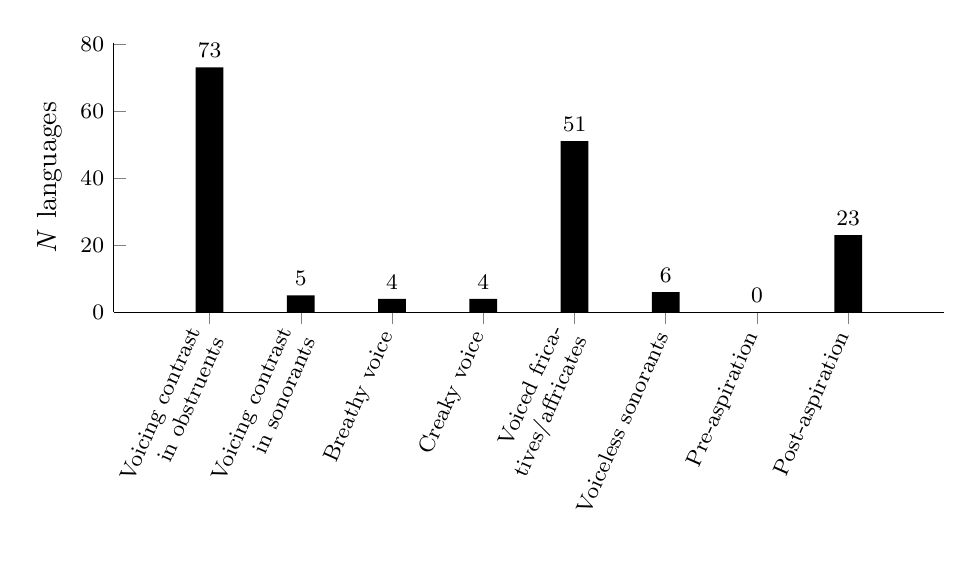
\begin{tikzpicture}
            \begin{axis}[
                    ybar,
                    ylabel={\textit{N} languages},
                    xtick=data,
                    axis lines*=left,
                    ymin=0,
                    scaled y ticks=false,
                    xticklabel style={font=\footnotesize,rotate=66, anchor=east, align=right,text width=2.5cm},
                    xticklabels = {{Voicing contrast in obstruents},{Voicing contrast in sonorants},{Breathy voice},{Creaky voice},{Voiced fricatives/affricates},{Voiceless sonorants},{Pre-aspiration},{Post-aspiration}},
                    ticklabel style={font=\footnotesize},
                    width=\textwidth,
                    height=5cm,
                    enlarge x limits={0.15},
                    nodes near coords,
                    nodes near coords style={text=black,font=\footnotesize},
                    ]
                \addplot+[
                     fill=black,draw=none
                    ] coordinates {(0,73) (1,5) (2,4) (3,4) (4,51) (5,6) (6,0) (7,23)};
%                   
\end{axis}
\end{tikzpicture}
\caption{\label{fig:4.4}Phonation features in consonant inventories, by number of languages in which they are present.}
\end{figure}

  Most of the phonation features examined here are found in ten or fewer languages. I briefly discuss those results here. None of the languages of the sample have \textit{pre-aspiration. Breathy voice} is present in only four languages: \ili{Darai}, \ili{Kharia}, \ili{Sumi Naga}, and \ili{Telugu}. All of these languages are from the Indian subcontinent, where this feature is prevalent (\citealt{LadefogedMaddieson1996}: 57--58). \textit{Creaky voice} occurs in four languages in the language sample. Here this term always refers to consonants described as glottalized sonorants which are often transcribed with an ejective or glottalization diacritic (e.g. /ɰ’/, /w\textsuperscript{ʔ}/). This feature is strongly associated with northern North America, occurring in \ili{Nuu-chah-nulth}, \ili{North Slavey}, and \ili{Thompson}, but also occurs in one language from Southeast Asia \& Oceania (\ili{Pacoh}). Finally, there are six languages with \textit{voiceless sonorants}: \ili{Hadza}, \ili{Kambaata}, \ili{Kunjen}, \ili{Nivkh}, \ili{Sichuan Yi}, and \ili{Southern Grebo}. In all of these except for \ili{Kunjen}, a \textit{voicing contrast in sonorants} occurs such that at least one pair of these consonants is distinguished solely by a modal voicing/voiceless contrast.

  There are three other phonation features -- \textit{voicing contrast in obstruents}, \textit{voiced fricatives/affricates}, and \textit{post-aspiration} -- which occur in more than ten languages each. \figref{fig:4.5} attempts to capture any trends that exist with respect to the presence of these features and syllable structure complexity. The figure shows the percentage of languages in each category of syllable structure which have the given phonation feature in their consonant inventories.

\begin{figure}
\begin{tikzpicture}
\pgfplotstableread{data/fig45.csv}{\table}
    \pgfplotstablegetcolsof{\table}
    \pgfmathtruncatemacro\numberofcols{\pgfplotsretval-1}
            \begin{axis}[easterdayline,ymax=100]
            \foreach \i in {1,...,\numberofcols} {
                \addplot+ table [x index={1},y index={\i},x expr=\coordindex] {\table};
                \pgfplotstablegetcolumnnamebyindex{\i}\of{\table}\to{\colname} % Adding column headers to legend
                \addlegendentryexpanded{\colname}
            }
            \end{axis}                                                                           
\end{tikzpicture}
\caption{\label{fig:4.5}Percentage of languages in each category of syllable structure complexity having the given phonation feature in their consonant inventories. For the calculation of the \textit{voiced fricatives/affricates} trend, four languages which have neither fricatives nor affricates have been excluded (see \sectref{sec:4.4.5})}.
\end{figure}

  Only the \textit{voicing contrast in obstruents} feature has a near-monotonic, albeit weak, trend with respect to syllable structure complexity. While having a voicing contrast in obstruents is the norm for languages in all four categories of syllable structure, this feature is found with the highest frequency in languages from the Simple category and with lowest frequency in languages from the Highly Complex category. This trend is no doubt strongly influenced by the high representation of languages from the Americas in this category. See \figref{fig:4.6} for a map of the geographical distribution of the languages lacking a voicing contrast in obstruents, which are heavily concentrated in the Americas. Most (6/9) of the languages without this feature in the Highly Complex category are from this region.

  
\begin{figure}
\includegraphics[width=\textwidth]{figures/fig46.png}
\caption{\label{fig:4.6}Areal distribution of languages in sample with no voicing contrast in obstruents.}
\end{figure}

  Indeed, the trend with respect to the \textit{voicing contrast in obstruents} feature is not significant in chi-square tests. Thus we do not find strong evidence for a relationship between phonation features and syllable structure complexity in this language sample.

\subsection{Place features}\label{sec:4.4.4}

  In this section I present an analysis of place features in the consonant phoneme inventories of the language sample. This analysis considers only the patterns of non-glide consonants. In \tabref{tab:4.13} I list the place features considered.

\begin{table}[t]
\begin{tabularx}{\textwidth}{QQ}
\lsptoprule
Basic & Elaborated\\\midrule
labial-velar

bilabial

dental

alveolar

dental/alveolar

alveolo-palatal

palatal

velar

glottal & labiodental

palato-alveolar

retroflex

uvular

pharyngeal

palatalization

labialization

pharyngealization

velarization\\
\lspbottomrule
\end{tabularx}
\caption{\label{tab:4.13}Basic and elaborated place features examined here.}
\end{table}

  \figref{fig:4.7} shows how many languages in the sample each place feature is found in. Note that in the figure I have merged languages which have dental, alveolar or dental/alveolar articulations into one category of \textit{dental/alveolar}. This is to distinguish languages reported to have only one of these places of articulation from those reported to have both dental and alveolar articulations (the \textit{dental and alveolar} category).


\begin{figure}[t]
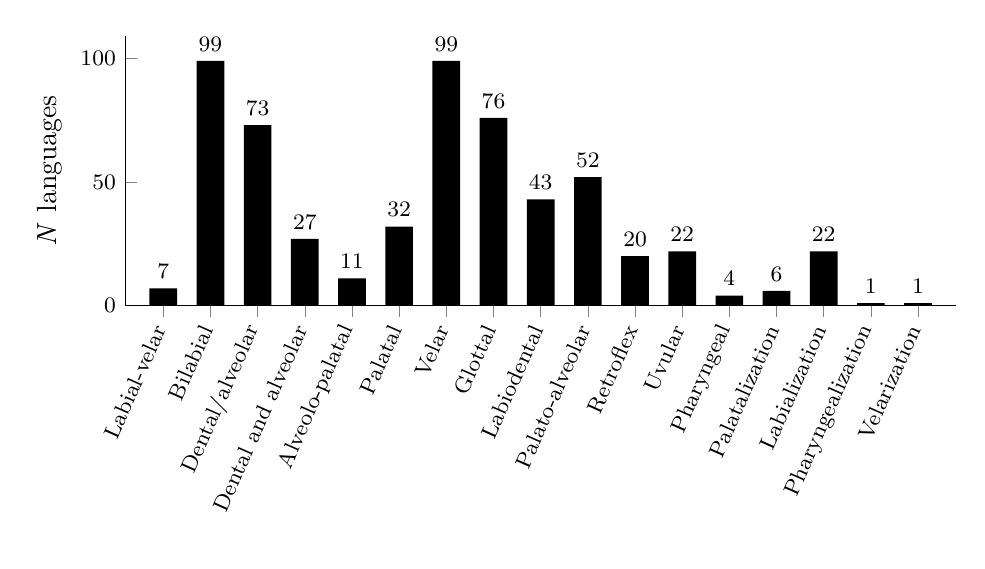
\begin{tikzpicture}
            \begin{axis}[
                    ybar,
                    ylabel={\textit{N} languages},
                    xtick=data,
                    axis lines*=left,
                    ymin=0,
                    scaled y ticks=false,
                    xticklabel style={font=\footnotesize,rotate=66, anchor=east, align=right,text width=2.75cm},
                    xticklabels = {{Labial-velar},{Bilabial},{Dental/alveolar},{Dental and alveolar},{Alveolo-palatal},{Palatal},{Velar},{Glottal},{Labiodental},{Palato-alveolar},{Retroflex},{Uvular},{Pharyngeal},{Palatalization},{Labialization},{Pharyngealization},{Velarization}},
                    ticklabel style={font=\footnotesize},
                    width=\textwidth,
                    height=5cm,
                    enlarge x limits={0.05},
                    nodes near coords,
                    nodes near coords style={text=black,font=\footnotesize},
                    ]
                \addplot+[
                     fill=black,draw=none
                    ] coordinates {(0,7) (1,99) (2,73) (3,27) (4,11) (5,32) (6,99) (7,76) (8,43) (9,52) (10,20) (11,22) (12,4) (13,6) (14,22) (15,1) (16,1) };
%                   
\end{axis}
\end{tikzpicture}
\caption{\label{fig:4.7}Place features in consonant inventories, by number of languages in which they are present.}
\end{figure}

  Several of the place features are (nearly) universal in the sample. All languages except for \ili{Mohawk} have \textit{bilabial} consonants, and all but \ili{Wutung} have \textit{velar} consonants. All languages in the sample have either \textit{dental/alveolar} or \textit{dental and alveolar} consonants; there is no trend with respect to syllable structure complexity for either of these features.

  There are five place features in the sample that are present in fewer than ten languages. The \textit{labial-velar} feature occurs in seven languages, six of which are spoken in Africa (\ili{Southern Bobo Madaré}, \ili{Doyayo}, \ili{Ewe}, \ili{Southern Grebo}, \ili{Lelepa}, \ili{Ma’di}, and \ili{Yoruba}). Secondary \textit{palatalization} is present in six languages (\ili{Cocopa}, \ili{Pinotepa Mixtec}, \ili{Polish}, \ili{Paiwan}, \ili{Towa}, and \ili{Urarina}). The remaining rare place features are found only in languages with Highly Complex syllable structure. Secondary \textit{pharyngealization} and \textit{velarization} are present in one language each (\ili{Tashlhiyt} and \ili{Albanian}, respectively). \textit{Pharyngeal} consonants are found in languages from areas which are famous ``hotspots'' of complex syllable structure: the Pacific Northwest (\ili{Nuu-chah-nulth}, \ili{Thompson}), the Caucasus (\ili{Kabardian}), and the Atlas Mountains (\ili{Tashlhiyt}).\footnote{{Here the term} \textrm{\textit{pharyngeal} }\textrm{also includes epiglottal consonants.}}

  The remaining eight place features -- \textit{labiodental}, \textit{alveolo-palatal, palato-alveo\-lar}, \textit{retroflex}, \textit{palatal}, \textit{uvular}, \textit{glottal}, and secondary \textit{labialization} -- are found in more than ten languages each. Of these, there are three features which show a \mbox{(near-)}\linebreak monotonic increase or decrease in frequency with respect to syllable structure complexity. These are shown in \figref{fig:4.8}.

\begin{figure}
\begin{tikzpicture}
\pgfplotstableread{data/fig48.csv}{\table}
    \pgfplotstablegetcolsof{\table}
    \pgfmathtruncatemacro\numberofcols{\pgfplotsretval-1}
            \begin{axis}[easterdayline,ymax=100]
            \foreach \i in {1,...,\numberofcols} {
                \addplot+ table [x index={1},y index={\i},x expr=\coordindex] {\table};
                \pgfplotstablegetcolumnnamebyindex{\i}\of{\table}\to{\colname} % Adding column headers to legend
                \addlegendentryexpanded{\colname}
            }
            \end{axis}                                                                           
\end{tikzpicture}
\caption{\label{fig:4.8}Percentage of languages in each category of syllable structure complexity having the given place feature.}
\end{figure}

  There are two features in \figref{fig:4.8} which show strong positive trends with respect to syllable structure complexity. \textit{Palato-alveolars}, which are generally frequent in the language sample, are strongly associated with Highly Complex syllable structure, though the trend in this feature is not strictly linear between the Simple to Complex categories. This trend is statistically significant: $\chi^2(3, N = 100) = 14.59$, $p = 0.002$. The \textit{uvular} pattern is especially striking. This place feature is distinctive in just one language (\ili{Sumi Naga}) from the Simple category, yet its frequency of occurrence rises monotonically with syllable structure complexity to the extent that nearly half of the languages with Highly Complex syllable structure have consonants at this place of articulation. This trend is highly significant: $\chi^2(3, N = 100) = 16.01$, $p = 0.001$. 

  The geographical distribution of uvulars is shown in \figref{fig:4.9}. While the prevalence of this feature in the Highly Complex syllable structure is boosted by its concentration in areas such as the Pacific Northwest and the Caucasus, it is notable that uvulars are also found to co-occur with Highly Complex syllable structure in regions as far-flung as New Guinea, Northeast Asia, and Patagonia.

\begin{figure}
\includegraphics[width=\textwidth]{figures/fig49.png}
\caption{\label{fig:4.9}Areal distribution of languages in sample with uvular consonants.}
\end{figure}

  The \textit{palatal} articulation shows a negative trend with respect to syllable structure complexity. While this trend is not significant in a chi-square test, it is interesting that it runs counter to that established for \textit{palato-alveolars}. This observation brings up an important issue of terminology and description. It is not uncommon for authors of language descriptions to use the term ``palatal'' in classifying the place of a series of consonants, but transcribe the consonants with the symbols used for palato-alveolars. Similarly, the terms ``alveolo-palatal'' and ``alveo-palatal'' may be used in prose descriptions, while palato-alveolar symbols are used in transcription. In her crosslinguistic study of palatalization, \citet{Bateman2007} notes that there is often disagreement on the transcription conventions used for secondarily palatalized velars, fronted velars, and palatal consonants. It is understandable that there is some inconsistency and interchangeability in the use of these terms: the area of contact between the tongue body and the hard palate may be large and variable in consonants articulated in this region, making it difficult to select a place classification (\citealt{LadefogedMaddieson1996}: 30--33). Since palato-alveolar and palatal places of articulation are not always reliably distinguished from one another or other similar articulations, we must consider the possibility that the trends with respect to these features in \figref{fig:4.8} effectively cancel each other out. In such a scenario, there would be no trend with respect to consonant articulations in this region of the vocal tract and syllable structure complexity.

  In order to clarify this issue, five places in the general region of the hard palate are examined: \textit{palato-alveolar}, \textit{palatal}, \textit{palatalized alveolar and/or velar}, and \textit{alveolo-palatal}. For each language, the number of places in which consonants are produced in this region is noted. For example, the phoneme inventory of \ili{Polish} has consonants in three distinct places in this region: palato-alveolar, alveolo-palatal, and palatalized velar \REF{ex:4.32}.

\ea\label{ex:4.32}
\etriple{Polish}{Indo-European}{Poland}
\begin{Coding}
\item[C phoneme inventory:] /p b pʲ bʲ t̪ d̪ k ɡ kʲ ɡʲ t̪͡s̪ d̪͡z̪ t͡ʃ d͡ʒ t͡ɕ d͡ʑ f v fʲ vʲ s̪ z̪ ʃ ʒ ɕ ʑ x m mʲ n̪ ɲ r l j w/
\end{Coding}
\z

  \figref{fig:4.10} shows the distribution of languages in the sample with respect to how many places are utilized in the region of the hard palate.

\begin{figure}
\caption{\label{fig:4.10} Number of place distinctions made in the region of the hard palate in languages with different syllable structure complexity. Place distinctions considered here are \textit{palato-alveolar}, \textit{palatal}, \textit{palatalized alveolar and/or velar}, and \textit{alveolo-palatal}. For each category of syllable structure complexity, I show the percentage of languages having one, two, three, or none of these places represented in their consonant inventories.}
\begin{tikzpicture}
\pgfplotstableread{data/fig410.csv}{\table}
    \pgfplotstablegetcolsof{\table}
    \pgfmathtruncatemacro\numberofcols{\pgfplotsretval-1}
            \begin{axis}[easterdaystacked,
                                xticklabels={S,MC,C,HC},
                        ]
            \foreach \i in {1,...,\numberofcols} {
                \addplot+[
                    /pgf/number format/read comma as period, fill
                    ] table [x index={1},y index={\i},x expr=\coordindex] {\table};
                \pgfplotstablegetcolumnnamebyindex{\i}\of{\table}\to{\colname} % Adding column headers to legend
                \addlegendentryexpanded{\colname}
            }
            \end{axis}                                                                           
\end{tikzpicture}
\end{figure}

  In all categories, most languages have at least one place articulation in the region of the hard palate. Crucially, the patterns in \figref{fig:4.10} show that the percentage of languages having one or more articulations in the region of the hard palate increases steadily with syllable structure complexity. That is, the trend favoring purported ``palatal'' articulations in languages with simpler syllable structure does not cancel out the trend favoring purported ``palato-alveolar'' articulations in languages with more complex syllable structure.

  Below I present another analysis of the proliferation of place distinctions in a large region of the vocal tract. In this case, the number of place distinctions made in the post-velar region is considered. The distinctions considered here are the \textit{uvular}, \textit{labialized uvular}, \textit{pharyngeal}, \textit{pharyngealized}, and \textit{glottal} places of articulation. \figref{fig:4.11} shows how the number of post-velar distinctions patterns with respect to syllable structure.

\begin{figure}
\caption{\label{fig:4.11} Number of place distinctions made in the post-velar region in languages with different syllable structure complexity. Place distinctions considered here are \textit{uvular}, \textit{labialized uvular}, \textit{pharyngeal, pharyngealization}, and \textit{glottal}. For each category of syllable structure complexity, I show the percentage of languages having 1, 2, ${\geq}$3, or none of these places represented in their consonant inventories.}
\begin{tikzpicture}
\pgfplotstableread{data/fig411.csv}{\table}
    \pgfplotstablegetcolsof{\table}
    \pgfmathtruncatemacro\numberofcols{\pgfplotsretval-1}
            \begin{axis}[easterdaystacked,
                                xticklabels={S,MC,C,HC},
                        ]
            \foreach \i in {1,...,\numberofcols} {
                \addplot+[
                    /pgf/number format/read comma as period, fill
                    ] table [x index={1},y index={\i},x expr=\coordindex] {\table};
                \pgfplotstablegetcolumnnamebyindex{\i}\of{\table}\to{\colname} % Adding column headers to legend
                \addlegendentryexpanded{\colname}
            }
            \end{axis}                                                                           
\end{tikzpicture}
\end{figure}

  In all categories of syllable structure complexity, roughly similar proportions of languages have at least one post-velar place of articulation, usually glottal. However, in the Complex and Highly Complex categories, one-fifth and one-half of languages, respectively, have consonants at more than one place in the post-velar region. In fact, in the Highly Complex category, some languages have consonant systems which make use of four post-velar places (\ili{Kabardian}, \ili{Nuu-chah-nulth}, and \ili{Thompson}), and one language (\ili{Tashlhiyt}) has consonants at all five post-velar places. Below I show the consonant phoneme inventory of \ili{Nuu-chah-nulth}, which has consonants at \textit{uvular}, \textit{labialized uvular}, \textit{pharyngeal}, and \textit{glottal} places of articulation \REF{ex:4.33}.

\ea\label{ex:4.33}
\etriple{Nuu-chah-nulth}{Wakashan}{Canada}
\begin{Coding}
\item[C phoneme inventory:] /p t k kʷ q qʷ ʕ ʔ p’ t’ k’ k’ʷ t͡s t͡ʃ t͡ɬ t͡s’ t͡ʃ’ t͡ɬ’ s ɬ ʃ x xʷ χ χʷ ħ h m n m’ n’ j w j’ w’/
\end{Coding}
\z

  In this section we have found that there are two place features of consonants which have statistically significant positive trends with respect to syllable structure complexity: \textit{uvular} and \textit{palato-alveolar} articulations (or at least one place in the region of the hard palate). Languages with more complex syllable structure also tend to have more consonant place articulations in the post-velar region, and infrequent post-velar articulations \textit{pharyngeal}, \textit{pharyngealization}, and \textit{velarization} are found only in languages with Highly Complex syllable structure in the current sample.

\subsection{Manner features}\label{sec:4.4.5}

  Here the manner features in the consonant phoneme inventories of the language sample are analyzed. In \tabref{tab:4.14} I list the manner features considered.

\begin{table}
\begin{tabularx}{\textwidth}{QQ}
\lsptoprule
{Basic} & {Elaborated}\\\midrule
stop

affricate

fricative

nasal

flap/tap

trill

central approximant

lateral affricate

lateral fricative

lateral flap

lateral approximant & prenasalization

nasal release

lateral release

ejective

implosive

click\\
\lspbottomrule
\end{tabularx}
\caption{\label{tab:4.14}Basic and elaborated manner features examined here. ``Central approximants'' include non-lateral approximants such as glides but also ``rhotic'' approximants like /ɹ/.}
\end{table}

  \figref{fig:4.12} shows how many languages in the sample have each manner feature. Because all instances of lateral release in the data were lateral affricates, these features have been merged so that only \textit{lateral release} is represented in the figure. \textit{Lateral flap} has also been merged with the more frequent (non-lateral) \textit{flap/tap} articulation.

  
\begin{figure}

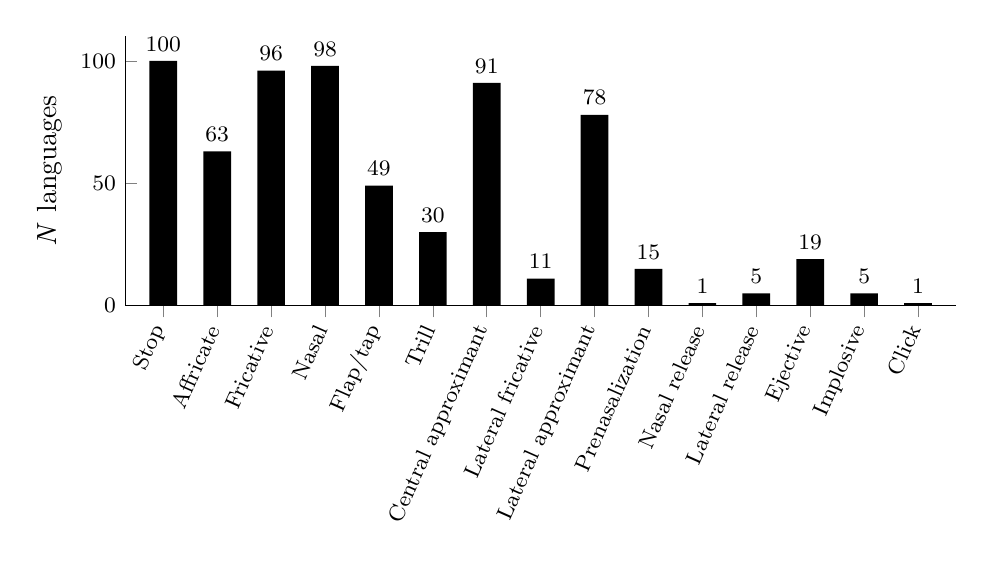
\begin{tikzpicture}
            \begin{axis}[
                    ybar,
                    ylabel={\textit{N} languages},
                    xtick=data,
                    axis lines*=left,
                    ymin=0,
                    scaled y ticks=false,
                    xticklabel style={font=\footnotesize,rotate=66, anchor=east, align=right,text width=2.75cm},
                    xticklabels = {{Stop},{Affricate},{Fricative},{Nasal},{Flap/tap},{Trill},{Central approximant},{Lateral fricative},{Lateral approximant},{Prenasalization},{Nasal release},{Lateral release},{Ejective},{Implosive},{Click}},
                    ticklabel style={font=\footnotesize},
                    width=\textwidth,
                    height=5cm,
                    enlarge x limits={0.05},
                    nodes near coords,
                    nodes near coords style={text=black,font=\footnotesize},
                    ]
                \addplot+[
                     fill=black,draw=none
                    ] coordinates {(0,100) (1,63) (2,96) (3,98) (4,49) (5,30) (6,91) (7,11) (8,78) (9,15) (10,1) (11,5) (12,19) (13,5) (14,1)};
%                   
\end{axis}
\end{tikzpicture}
\caption{\label{fig:4.12} Manner features in consonant inventories, by number of languages in which they are present.}
\end{figure}

  As with place features, there are several manner features which are (nearly) universal in the sample. \textit{Stops} occur in every language. \textit{Nasals} occur in all but two languages (\ili{Cubeo} and \ili{Rotokas}). There are four languages lacking \textit{fricatives}: \ili{Alyawarra}, \ili{Bardi}, \ili{Mangarrayi}, and \ili{Ngarinyin}. All of these languages are spoken in Australia, a region where this rare typological feature is common \citep[42]{Maddieson1984}. \textit{Central approximants} are reported to be absent in nine languages. However, in at least some of these languages, phonetic glides occur in complementary distribution with other sounds (e.g. \ili{Urarina}, \citealt{Olawsky2006}: 37).

  There are five manner features occurring in ten or fewer languages in the sample. \textit{Clicks} and \textit{nasal release} occur in one language each (\ili{Hadza} and \ili{Alyawarra}, respectively). \textit{Implosives} are present in the consonant inventories of five languages, all from Africa and Southeast Asia \& Oceania: \ili{Doyayo}, \ili{Tukang Besi}, Sre, \ili{Ma’di}, and \ili{Mpade}. \textit{Lateral release}, which corresponds to lateral affricates, is found in only five languages, mostly from North America: \ili{Hadza}, \ili{Nuu-chah-nulth}, \ili{North Slavey}, \ili{Thompson}, and \ili{Yakima Sahaptin}.

  The remaining seven manner features considered here -- \textit{affricate}, \textit{flap/tap}, \textit{trill}, \textit{lateral fricative}, \textit{lateral approximant}, \textit{ejective}, \textit{prenasalization} -- occur in more than ten languages each. Three of these --  \textit{flap/tap}, \textit{prenasalization}, and \textit{ejective} -- show a (near-)monotonic increase or decrease with respect to syllable structure complexity. While the feature \textit{affricate} does not show a linear trend, it does show a large overall increase in frequency between the Simple and Highly Complex categories. The patterning of these four features with respect to syllable structure complexity can be found in \figref{fig:4.13}.

\begin{figure}
\begin{tikzpicture}
\pgfplotstableread{data/fig413.csv}{\table}
    \pgfplotstablegetcolsof{\table}
    \pgfmathtruncatemacro\numberofcols{\pgfplotsretval-1}
            \begin{axis}[easterdayline,ymax=100]
            \foreach \i in {1,...,\numberofcols} {
                \addplot+ table [x index={1},y index={\i},x expr=\coordindex] {\table};
                \pgfplotstablegetcolumnnamebyindex{\i}\of{\table}\to{\colname} % Adding column headers to legend
                \addlegendentryexpanded{\colname}
            }
            \end{axis}                                                                           
\end{tikzpicture}
\caption{\label{fig:4.13}Percentage of languages in each category of syllable structure complexity having the given manner feature.}
\end{figure}

  There are two manner features whose frequency in inventories is associated with increasing syllable structure complexity. The trend in \textit{affricates}, though not linear, is nevertheless significant: $\chi^2(3, N = 100) = 8.89$, $p = 0.03$. The \textit{ejectives} trend is statistically significant when the data from the Simple and Moderately Complex categories is combined and compared against that of the Complex and Highly Complex categories combined ($p =0.006$ in Fisher’s exact test). There is a heavy areal distribution of this feature: over half (10/19) of the languages with ejectives in the sample are found in the Americas. Outside the Americas, ejectives are also found to co-occur with Highly Complex syllable structure in the Caucasus region, Ethiopian Highlands, and Northeast Asia (see \figref{fig:4.14}).
\vfill
\begin{figure}  
\includegraphics[width=\textwidth]{figures/fig414.png}
\caption{\label{fig:4.14}Areal distribution of languages in sample with ejective consonants.}
\end{figure}
\vfill\pagebreak

  The proportion of languages with \textit{prenasalization} contrasts in their consonant phoneme inventories decreases with syllable structure complexity, though this trend is not statistically significant in a chi-square test. This trend is not clearly driven by any particular regional patterns: while roughly half (7/15) of languages with these articulations are from the region of Australia \& New Guinea, the distribution of those languages among the categories of syllable structure complexity is even. Further, the trend favoring prenasalization in languages with Simple syllable structure is not limited to a single region. The seven languages with Simple syllable structure and prenasalization are from four different macro-areas: Africa (\ili{Hadza}, \ili{Ma’di}), Australia \& New Guinea (\ili{East Kewa}, \ili{Savosavo}), North America (\ili{Pinotepa Mixtec}), and Southeast Asia \& Oceania (\ili{Tukang Besi}, \ili{Sichuan Yi}). It is interesting to note that, like Simple syllable patterns, prenasalization contrasts tend to be found in languages spoken in close proximity to the equator (\figref{fig:4.15}).


\begin{figure}  
\includegraphics[width=\textwidth]{figures/fig415.png}
\caption{\label{fig:4.15}Areal distribution of languages in sample with prenasalized consonants.}
\end{figure}

  The \textit{flap/tap} feature also has a negative relationship with syllable structure complexity in the language sample, although this trend is not statistically significant in a chi-square test. Examining the geographical distribution of languages with flap or tap articulations, we find that this trend can be found within most of the macro-areas in the sample (\figref{fig:4.16}).


\begin{figure}  
\includegraphics[width=\textwidth]{figures/fig416.png}
\caption{\label{fig:4.16}Areal distribution of languages in sample with flap/tap consonants.}
\end{figure}

  Flap and tap articulations differ from trill articulations in important ways. Flaps and taps are produced with a single rapid movement of the active articulator, usually the tongue tip, making brief contact with the passive articulator, usually the alveolar ridge. Trills in the coronal region often have the same configuration of articulators, but the movement of the active articulator is a vibration driven by aerodynamic currents rather than muscular movements (\citealt{LadefogedMaddieson1996}: 217--232). However, taps and flaps can vary allophonically with trills in some languages. We must allow for the possibility that the trend noted above reflects an analytical preference, in languages with simpler syllable structure, by which the flap/tap articulation is considered primary in such cases of allophonic variation. \figref{fig:4.17} shows how flap/tap and coronal trill articulations are distributed among languages with different syllable structure complexity. Even in the most liberal interpretation of the analytical preference scenario, the pattern with trill articulations does not clearly neutralize the pattern of flap/tap articulations.

\begin{figure}
\begin{tikzpicture}
\pgfplotstableread{data/fig417.csv}{\table}
    \pgfplotstablegetcolsof{\table}
    \pgfmathtruncatemacro\numberofcols{\pgfplotsretval-1}
            \begin{axis}[easterdaystacked,
                                xticklabels={S,MC,C,HC},
                        ]
            \foreach \i in {1,...,\numberofcols} {
                \addplot+[
                    /pgf/number format/read comma as period, fill
                    ] table [x index={1},y index={\i},x expr=\coordindex] {\table};
                \pgfplotstablegetcolumnnamebyindex{\i}\of{\table}\to{\colname} % Adding column headers to legend
                \addlegendentryexpanded{\colname}
            }
            \end{axis}                                                                           
\end{tikzpicture}
\caption{\label{fig:4.17} Distribution of languages with flap/tap and trill articulations, by syllable structure complexity.}
\end{figure}

  In this section we have found statistically significant trends positively associating \textit{affricate} and \textit{ejective} manners of articulation with syllable structure complexity. We also find weaker trends which are not statistically significant showing a negative association between the presence of \textit{flap/tap} and \textit{prenasalized} articulations and syllable structure complexity.

\subsection{Summary of consonant patterns in sample}\label{sec:4.4.6}

  Three hypotheses were formulated in \sectref{sec:4.1.4} with respect to consonant inventory patterns and syllable structure complexity. First, it was hypothesized that consonant phoneme inventory size would increase with syllable structure complexity. This relationship was upheld in the current sample and was found to be statistically significant. Second, it was hypothesized that the number of elaborated articulations present in consonant phoneme inventories would increase with syllable structure complexity. As expected, this correlation was found to be positive and significant, though the difference in average number of elaborations was not dramatic between the categories at the two extremes of syllable structure complexity. Finally, it was hypothesized that languages with more complex syllable structure would have different kinds of consonants in their inventories than languages with simpler syllable structure. The results of the analyses in \sectref{sec:4.4.3}--\ref{sec:4.4.5} suggest that this is the case, as there are specific consonant articulations which are more frequently present in languages of the Complex and Highly Complex categories. However, it was also found that there are consonant types which occur more frequently in languages with simpler syllable structures. Thus it can be said, more generally, that languages with different syllable patterns also tend to have different kinds of consonants in their phoneme inventories.

  Trends positively associating \textit{uvular}, \textit{palato-alveolar}, \textit{affricate}, and \textit{ejective} articulations with syllable structure complexity were found to be statistically significant in the current language sample, while trends negatively associating a \textit{voicing contrast in obstruents}, \textit{palatals}, \textit{flaps/taps} and \textit{prenasalization} with syllable complexity were not found to be statistically significant. However, given the relatively small sample size considered, it is possible that different results might be found for all of these trends in a larger sample. The robustness of each of these trends was investigated in the 501-language LAPSyD sample \citep{MaddiesonEtAl2013}. Within LAPSyD, it was found that most of these articulations -- all except for \textit{voicing contrast in obstruents} and \textit{palatals} -- have weak but highly significant positive or negative correlations with syllable structure complexity (measured as the sum of maximal syllable margins). These verified correlations, which correspond in directionality to those patterns established above, are listed and marked by asterisks in \tabref{tab:4.15}. Additionally, the table lists in italics two general trends established in the present study with respect to articulations in the palatal and postvelar regions.

\begin{table}
\begin{tabular}{>{\raggedright}p{1.5cm}lS[table-format=1.3]S[table-format=<1e1]}
\lsptoprule

{Type of feature} & {Articulation} & \multicolumn{2}{c}{Correlation in LAPSyD}\\\cmidrule(lr){3-4}
                  &                &  {$r(501)$}      &   {$p$}\\\midrule
{Place} & *Palato-alveolar & .162 & <5e-04\\
        & *Uvular  & .282 & <1e-05\\
& \textit{At least one distinction in palatal region} & \\
& \textit{More post-velar distinctions} &\\
{Manner} & *Affricate & .156 & <5e-04\\
         & *Ejective  & .180 & <1e-04\\
         & *Flap/tap  & -.136 & .002\\
         & *Prenasalization & -.175 & <1e-04\\
\lspbottomrule
\end{tabular}
\caption{\label{tab:4.15}Features of consonantal systems associated positively or negatively with syllable structure complexity. Where relevant, the statistically significant correlation in LAPSyD \citep{MaddiesonEtAl2013} is given.%%\todo[inline]{Is the remark in italics placed correctly?}
}
\end{table}

  There is an important general observation to be made regarding the patterns uncovered here. This is that the three standard aspects of consonant articulation examined here -- phonation, place, and manner -- pattern differently with respect to syllable structure complexity. Phonation features do not seem to be correlated with syllable structure complexity. The presence of certain place features is associated with more complex syllable structure. Both ends of the syllable structure complexity scale are associated with specific manner features, but very different kinds. The manners of articulation associated with more complex syllable structure (affricates and ejectives) are obstruents, while the manner features associated with simpler syllable structure are either sonorants (flap/tap), or arguably have a sonorant component (prenasalized consonants). These patterns may have important implications for uncovering the development of highly complex syllable structure, as well as for establishing a syllable structure-based phonological typology of languages. These issues will be discussed further in \sectref{sec:4.5}.

\section{Discussion}\label{sec:4.5}
\subsection{Segmental inventory patterns and syllable structure complexity}\label{sec:4.5.1}

  In light of the findings presented in the current chapter, we revisit the first broad research goal of this work, which is to determine whether languages with highly complex syllable structure share other characteristics such that this group can be classified as a holistic language type.

  The results indicate that there are a number of specific segmental patterns associated with highly complex syllable structure, all of which are related to consonants. These are summarized in \REF{ex:4.34}. The terms ``absence'' and ``presence'' are used here not in a categorical sense, but to mean relative absence or presence of a property in the Highly Complex group as compared to the other syllable structure complexity groups.

\ea\label{ex:4.34}
  Segmental patterns associated with Highly Complex category

\textit{Mean of 26 consonant phonemes}

\textit{Mean of 4 elaborations in consonant phoneme inventory}

\textit{Absence of prenasalized consonants}

\textit{Absence of flap/tap consonants}

\textit{Presence of palato-alveolar consonants}

\textit{Presence of uvular consonants}

\textit{Presence of affricate consonants} 

\textit{Presence of ejective consonants}
\z

  This list does not include two more general segmental patterns of languages with Highly Complex syllable structure: at least one place distinction in the region of the hard palate, and a more richly elaborated set of place distinctions in the post-velar region.

  Recall the analyses in \sectref{sec:3.4.1}--\ref{sec:3.4.2} which established two different distributions in the languages of the Highly Complex category. In eight languages -- \ili{Cocopa}, \ili{Georgian}, \ili{Itelmen}, \ili{Polish}, \ili{Tashlhiyt}, \ili{Thompson}, \ili{Tohono O’odham}, and \ili{Yakima Sahaptin} -- Highly Complex structures were found to be a prevalent pattern. In six languages -- \ili{Alamblak}, \ili{Bench}, \ili{Doyayo}, \ili{Kunjen}, \ili{Menya}, and \ili{Wutung} -- Highly Complex structures were found to be a minor pattern. As discussed in \chapref{sec:3}, the languages within each of these groups share similar patterns with respect to the occurrence of Highly Complex structures at each syllable margin, restrictions on consonant combinations in these structures, and the relative frequency of these structures. The 11 languages which belong to neither group -- \ili{Albanian}, \ili{Camsá}, \ili{Kabardian}, \ili{Lezgian}, \ili{Mohawk}, \ili{Nuu-chah-nulth}, \ili{Passamaquoddy-Maliseet}, \ili{Yine}, \ili{Qawasqar}, \ili{Semai}, and \ili{Tehuelche} -- have syllable patterns which vary with respect to the different features examined or which fall somewhere in between the patterns of the two extreme groups.

  It is reasonable to expect that if highly complex syllable structure has other phonetic and phonological correlates, then languages which differ in the extent to which these syllable structures are prominent might also exhibit the other correlates to different degrees. In \tabref{tab:4.16} the languages of the Highly Complex portion of the sample are divided into the three groups described above. The properties of vowel and consonant inventories associated with Highly Complex syllable structure and listed in \REF{ex:4.34} above are given in the columns. A check mark indicates that a language has the expected property; a shaded cell indicates that it does not. For consonant phoneme inventory size and number of elaborations, I have designated a value greater than or equal to the mean for the category to be the expected property.

\begin{table}
\begin{tabularx}{\textwidth}{lCCCCCCCC}
\lsptoprule
 & \rotatebox{90}{{\textbf{${\geq}$ 26} Cs}} & \rotatebox{90}{{\textbf{${\geq}$ 4} elabs.}} & \rotatebox{90}{\parbox{2.5cm}{Prenasalization\newline absent}} & \rotatebox{90}{{Flap\slash tap absent}} & \rotatebox{90}{\parbox{2.5cm}{Palato-alveolar\newline present}} & \rotatebox{90}{{Uvular present}} & \rotatebox{90}{\parbox{1.6cm}{Affricate\newline present}} & \rotatebox{90}{\parbox{1.6cm}{Ejective\newline present}}\\\midrule
& \multicolumn{8}{c}{Languages with prevalent Highly Complex patterns}\\\midrule
 \ili{Cocopa} & \cellcolor{lsLightGray} & \ding{51} & \ding{51} & \ding{51} & \ding{51} & \ding{51} & \ding{51} & \cellcolor{lsLightGray}\\
 \ili{Georgian} & \ding{51} & \ding{51} & \ding{51} & \cellcolor{lsLightGray} & \ding{51} & \ding{51} & \ding{51} & \ding{51}\\
 \ili{Itelmen} & \cellcolor{lsLightGray} & \ding{51} & \ding{51} & \ding{51} & \ding{51} & \ding{51} & \ding{51} & \ding{51}\\
 \ili{Polish} & \ding{51} & \ding{51} & \ding{51} & \ding{51} & \ding{51} & \cellcolor{lsLightGray} & \ding{51} & \cellcolor{lsLightGray}\\
 \ili{Tashlhiyt} & \ding{51} & \ding{51} & \ding{51} & \ding{51} & \ding{51} & \ding{51} & \cellcolor{lsLightGray} & \cellcolor{lsLightGray}\\
 \ili{Thompson} & \ding{51} & \ding{51} & \ding{51} & \ding{51} & \ding{51} & \ding{51} & \ding{51} & \ding{51}\\
 T. O’odham & \cellcolor{lsLightGray} & \cellcolor{lsLightGray} & \ding{51} & \cellcolor{lsLightGray} & \ding{51} & \cellcolor{lsLightGray} & \ding{51} & \cellcolor{lsLightGray}\\
 Y. Sahaptin & \ding{51} & \ding{51} & \ding{51} & \ding{51} & \ding{51} & \ding{51} & \ding{51} & \ding{51}\\\midrule
& \multicolumn{8}{c}{Languages with intermediate Highly Complex patterns}\\\midrule
 \ili{Albanian} & \ding{51} & \ding{51} & \ding{51} & \cellcolor{lsLightGray} & \ding{51} & \cellcolor{lsLightGray} & \ding{51} & \cellcolor{lsLightGray}\\
 \ili{Camsá} & \cellcolor{lsLightGray} & \cellcolor{lsLightGray} & \ding{51} & \cellcolor{lsLightGray} & \ding{51} & \cellcolor{lsLightGray} & \ding{51} & \cellcolor{lsLightGray}\\
 \ili{Kabardian} & \ding{51} & \ding{51} & \ding{51} & \ding{51} & \ding{51} & \ding{51} & \ding{51} & \ding{51}\\
 \ili{Lezgian} & \ding{51} & \ding{51} & \ding{51} & \ding{51} & \ding{51} & \ding{51} & \ding{51} & \ding{51}\\
 \ili{Mohawk} & \cellcolor{lsLightGray} & \cellcolor{lsLightGray} & \ding{51} & \ding{51} & \ding{51} & \cellcolor{lsLightGray} & \ding{51} & \cellcolor{lsLightGray}\\
 Nuuchahnulth & \ding{51} & \ding{51} & \ding{51} & \ding{51} & \ding{51} & \ding{51} & \ding{51} & \ding{51}\\
 P.-Maliseet & \cellcolor{lsLightGray} & \cellcolor{lsLightGray} & \ding{51} & \ding{51} & \ding{51} & \cellcolor{lsLightGray} & \ding{51} & \cellcolor{lsLightGray}\\
 \ili{Yine} & \cellcolor{lsLightGray} & \cellcolor{lsLightGray} & \ding{51} & \cellcolor{lsLightGray} & \ding{51} & \cellcolor{lsLightGray} & \ding{51} & \cellcolor{lsLightGray}\\
 \ili{Qawasqar} & \cellcolor{lsLightGray} & \cellcolor{lsLightGray} & \ding{51} & \ding{51} & \cellcolor{lsLightGray} & \ding{51} & \ding{51} & \ding{51}\\
 \ili{Semai} & \cellcolor{lsLightGray} & \cellcolor{lsLightGray} & \ding{51} & \cellcolor{lsLightGray} & \cellcolor{lsLightGray} & \cellcolor{lsLightGray} & \cellcolor{lsLightGray} & \cellcolor{lsLightGray}\\
 \ili{Tehuelche} & \cellcolor{lsLightGray} & \cellcolor{lsLightGray} & \ding{51} & \ding{51} & \ding{51} & \ding{51} & \ding{51} & \ding{51}\\\midrule
& \multicolumn{8}{c}{Languages with minor Highly Complex patterns}\\\midrule
 \ili{Alamblak} & \cellcolor{lsLightGray} & \cellcolor{lsLightGray} & \ding{51} & \cellcolor{lsLightGray} & \ding{51} & \cellcolor{lsLightGray} & \ding{51} &\cellcolor{lsLightGray} \\
 \ili{Bench} & \ding{51} & \cellcolor{lsLightGray} & \ding{51} & \cellcolor{lsLightGray} & \ding{51} & \cellcolor{lsLightGray} & \ding{51} & \ding{51}\\
 \ili{Doyayo} & \cellcolor{lsLightGray} & \cellcolor{lsLightGray} & \ding{51} & \cellcolor{lsLightGray} & \cellcolor{lsLightGray} & \cellcolor{lsLightGray} & \cellcolor{lsLightGray} & \cellcolor{lsLightGray}\\
 \ili{Kunjen} & \cellcolor{lsLightGray} & \ding{51} & \ding{51} & \ding{51} & \cellcolor{lsLightGray} & \cellcolor{lsLightGray} & \cellcolor{lsLightGray} & \cellcolor{lsLightGray}\\
 \ili{Menya} & \cellcolor{lsLightGray} & \ding{51} & \cellcolor{lsLightGray} & \ding{51} & \ding{51} & \ding{51} & \ding{51} & \cellcolor{lsLightGray}\\
 \ili{Wutung} & \cellcolor{lsLightGray} & \cellcolor{lsLightGray} & \ding{51} & \ding{51} & \ding{51} & \cellcolor{lsLightGray} & \ding{51} & \cellcolor{lsLightGray}\\
\lspbottomrule
\end{tabularx}
\caption{\label{tab:4.16}Highly Complex languages, divided into three groups according to the prominence of their Highly Complex patterns. Check mark indicates that the given language has the expected segmental property; shaded cell indicates it does not.}
\end{table}

  The visual pattern in \tabref{tab:4.16} indicates that the expectations are borne out. Languages which have Highly Complex syllable structure as a prevalent pattern also tend to have more of the established segmental correlates of Highly Complex syllable structure. Languages which have Highly Complex syllable structure as a minor pattern tend to have fewer of the segmental correlates. The ``intermediate'' languages have a pattern that is intermediate between the two. It is striking that the three subtypes of Highly Complex syllable structure, which were defined entirely by reference to their syllable patterns, show the predicted patterns with respect to the presence of segmental correlates of Highly Complex syllable structure.

  Five languages have all of the established segmental correlates of Highly Complex syllable structure. Their consonant inventories might be considered to be prototypical of the Highly Complex category. To illustrate, I give the consonant inventory of \ili{Yakima Sahaptin} in \REF{ex:4.35}.

\ea\label{ex:4.35}
\etriple{Yakima Sahaptin}{Sahaptin}{USA}
\begin{Coding}
\item[C phoneme inventory:] /p t k kʷ q qʷ ʔ p’ t’ k’ k’ʷ q’ q’ʷ t͡ɬ t͡s t͡ʃ t͡ɬ’ t͡s’ t͡ʃ’ ɬ s ʃ x xʷ χ χʷ h m n l w j/
\end{Coding}
\z

  The results of the analyses in this chapter also reveal tendencies in the segmental patterns of languages on the Simple end of the syllable structure complexity cline. In most cases these patterns are the opposite of those consonantal properties given in \REF{ex:4.34} for the Highly Complex category. However, some of the segmental patterns observed in this category are more extreme than others. In the case of uvulars and ejectives, there is a near absence of this consonant type in languages with Simple syllable structure. Additionally, there are three segmental properties of vowels, including the absence of a length contrast of vowels, the presence of a nasalization contrast in vowels, and the presence of a vowel phonation contrast, which show patterns favoring Simple syllable structure. Finally, languages with Simple syllable structure have the lowest mean number of consonant phonemes (21 consonants) of all the categories examined here.

  It is important to keep in mind that the findings reported here are tendencies, some of them quite subtle. Languages in the sample also show wide variation in the structuring of their segmental inventories, resulting in many exceptions to the general patterns. \ili{Hadza} is in the Simple category, yet has the largest consonant inventory and number of elaborations of all the languages.\footnote{Borrowing may account for some of the sounds in the \ili{Hadza} phoneme inventory. Bonny Sands\ia{Sands, Bonny@Sands, Bonny} (p.c.) notes that it is possible that some click articulations have been borrowed from other click languages, in the same way that some Bantu languages have borrowed clicks from neighboring Khoisan languages. Kirk Miller\ia{Miller, Kirk@Miller, Kirk} (p.c.) suggests that \ili{Hadza} seems to have borrowed its initial prenasalized consonants and all voiced obstruents besides /b/. Even excluding clicks and non-bilabial voiced obstruents, the language would have a consonant inventory of 41 segments, which is still quite large. Sands and Miller agree that, apart from the presence of clicks, the phoneme inventory of \ili{Hadza} is not atypical for an East African, and particularly Cushitic, language.} \ili{Mohawk} and Passamaquoddy-Maliseeet are in the Highly Complex category, yet have very small consonant inventories and few articulatory elaborations. However, it is encouraging for the wider implications of this study that several of the general findings, such as those regarding consonant phoneme inventory size and consonant elaborations, replicate the results of previous studies with much larger sample sizes or can be verified in LAPSyD (\citealt{MaddiesonEtAl2013}, 501 languages). It is also notable that the distribution of features correlated with languages at either end of the syllable structure complexity cline does not appear to be random. The Highly Complex category is coherently associated with a group of consonant place features and manner features related to obstruents. The Simple category is coherently associated with two manner features related to sonorants. This point will be discussed further in the following sections.

  Having established segmental correlates of syllable structure complexity, we revisit the second research question of the book: how does highly complex syllable structure develop over time? The segment inventory of a language reflects, at least in part, sound changes which occurred at some point in the history of the language. Some typologically frequent speech sounds -- for instance, voiceless stops at labial, dental/alveolar, and velar places of articulation -- tend to persist within sound systems over the history of a language, and are not often observed to come about from other sounds as the result of allophonic processes (\citealt{Bybee2015a}; see also discussion in \sectref{sec:4.1.1}). This tendency may reflect general biological constraints on the vocal tract and/or the perceptual robustness of these sounds. However, for many other sounds, there is evidence for how they tend to develop through phonetic mechanisms in language use. 

  In \sectref{sec:4.5.2} I discuss reported processes of sound change which result in the consonantal patterns associated with Highly Complex syllable structure. In \sectref{sec:4.5.3} I discuss reported processes resulting in the consonantal patterns associated with Simple syllable structure. In the following I include historical, comparative, and synchronic accounts of sound change processes. Although historical evidence is best because it involves more or less direct observation, the history of written language is such that there are very few languages, language families, and regions for which such evidence exists on a deep time scale. Including reports of synchronic and comparative processes greatly expands the range of data available, but it does come with the caveat that the reported patterns may have other possible analyses. Many of the synchronic processes reported here are from AlloPhon, a database of over 800 phonetically-conditioned processes in 81 diverse languages (\citealt{BybeeEasterday2019}).

  In \sectref{sec:4.5.4}, I compare the patterns reported in \sectref{sec:4.5.2}--\ref{sec:4.5.3} and discuss their broad implications with respect to the diachronic development of highly complex syllable structure and syllable typology more generally.

\subsection{Articulations and contrasts characteristic of the Highly Complex category} \label{sec:4.5.2}

  In this section I present historical, comparative, and synchronic accounts of processes resulting in articulations and contrasts associated with the Highly Complex category, specifically palato-alveolars, uvulars, ejectives, and affricates. Additionally, as a more richly elaborated set of post-velar consonant distinctions is associated with this category, I also discuss the historical development of pharyngeals. As will be discussed in \sectref{sec:4.5.4}, all of these articulations commonly result from the place assimilation of consonants to vowels and strengthening processes.

\subsubsection{{Palato-alveolars}}\label{sec:4.5.2.1}

  Palato-alveolars are articulations made with the tongue blade in the area of the hard palate behind the alveolar ridge. These are known to develop from many different kinds of consonants. The most common conditioning environments for the development of these sounds are front, especially high front, vowels and palatal glides. Thus palato-alveolars are often a product of the crosslinguistically common process of palatalization (\citealt{Bhat1978}; \citealt{Bateman2007,BybeeEasterday2019}). Typically, the consonant undergoing palatalization precedes the conditioning vowel or glide. In a common type of process, palato-alveolars may develop out of alveolar consonants preceding a high front vowel, as in synchronic processes in \ili{Cantonese} \REF{ex:4.36} and \ili{Logba} \REF{ex:4.37}.

\ea\label{ex:4.36}
  \etriple{Cantonese}{Sino-Tibetan}{China}
\gll /t͡sy/\\
[t͡ʃy]\\
\glt ‘live’ (\citealt{MatthewsYip1994}: 14)
\z

\ea\label{ex:4.37}
  \etriple{Logba}{Atlantic-Congo}{Ghana}
\gll /onziɛ/\\
[onʒiɛ]\\
\glt ‘owl’ \citep[18]{Dorvlo2008}
\z

  Palato-alveolars are also known to develop out of velar consonants. The usual situation involves a velar stop becoming a palato-alveolar affricate preceding a high front vowel or glide. A well-known example of this occurred in the late stages of \ili{Latin} and early stages of Romance, when velar stops were fronted preceding front vowels, then eventually became palato-alveolar affricates in some of the daughter languages, e.g. \ili{Latin} [k]\textit{ivitate} > \ili{Italian} [t͡ʃ]\textit{ittà} ‘city’ \citep[113]{Posner1996}. \citet{Bhat1978} lists many examples, mostly historical, of velar palatalization resulting in palato-alveolar affricates preceding front vowels.

  Synchronic instances of velar palatalization resulting in palato-alveolar affricates are relatively rare: in the AlloPhon database, there is only one phonet\-ic\-al\-ly-conditioned process fitting this description out of approximately 50 palatalization processes in 45 languages (\citealt{BybeeEasterday2019}). \citet{Bateman2007} reports a higher proportion of such processes in her survey of 58 languages with palatalization, though she additionally considers morphophonological processes. These facts suggest that the palato-alveolar outcome from velars typically follows a long chain of incremental palatalization in the history of a language.

  More rarely, palato-alveolar consonants may develop from glide strengthening. This is the process by which a glide becomes more constricted in its articulation, sometimes becoming a fricative, affricate, or even a stop. This typically occurs in syllable-initial position (\citealt{BybeeEasterday2019}). A process of this sort has occurred recently in Argentinean \ili{Spanish}, where the sound corresponding to palatal approximant /j/ in other major dialects is now realized as [ʃ] or [ʒ], among other obstruent variants, in syllable-initial position: e.g. Castilian \ili{Spanish} \textit{a}[j]\textit{er} corresponds to Argentinean \ili{Spanish} \textit{a}[ʒ]\textit{er}{\textasciitilde} \textit{a}[ʃ]\textit{er} ‘yesterday’ (\citealt{HarrisKaisse1999}: 118).

  Very rarely, palato-alveolars may develop out of labial consonants. Such a process can be found in \ili{Romanian}; e.g. Standard \ili{Romanian} /fjer/ corresponds to \ili{Moldavian} /ʃer/ ‘iron’ \citep[108]{Bateman2007}. Bateman argues that full palatalization of labial consonants is better analyzed as a strengthening of the palatal articulation following the labial, and subsequent weakening and deletion of the labial gesture. In her sample, labial palatalization always occurs in specific morphophonological contexts, and is always the outcome of a series of historical developments. \citet{Ohala1978} argues for a perceptual basis for a similar phenomenon of full palatalization of labials in Southern Bantu, noting that labial-palatal sequences can be misperceived as palato-alveolar consonants.

  Palato-alveolars may also develop out of alveolars with secondary palatalization, as in the example of free variation in \ili{Dan} \REF{ex:4.38}.

\ea\label{ex:4.38}
\etriple{Dan}{Mande}{Côte d’Ivoire, Guinea, Liberia}
\gll /sʲa\textsuperscript{5}/\\
[sʲa\textsuperscript{5}]{\textasciitilde}[ʃa\textsuperscript{5}]\\
\glt ‘to indicate’ (\citealt{BearthZemp1967}: 17)
\z

Like the glide strengthening and velar fronting and affrication processes described above, the process in \ili{Dan} appears to be the end result of a chain of palatalization processes. The presence of consonant phonemes with secondary palatalization implies that palatalization has a long history in the language.

  Finally, palato-alveolars may develop out of free variation with other sounds having a palatal articulation. \citet[31--33]{LadefogedMaddieson1996} note that palatal stops are often produced with affrication due to the large surface area required for stop in this region, and as a result may vary with palato-alveolar affricates in a language.

  The free variation of palatal stops with palato-alveolar affricates can be seen as a weakening of the abrupt stop release, and therefore a case of lenition. However, we find that the most common sound change processes leading to the development of palato-alveolar consonants are assimilation, usually anticipatory, to a high and/or front vowel or glide, and fortition of palatal glides. Both articulatory and perceptual accounts have been put forward to account for the high crosslinguistic frequency of these palatalization processes. Fronted velar stops and palato-alveolar affricates have acoustic similarities in their release bursts, which has led some to argue that this sound change is a result of perceptual reanalysis \citep{Guion1998}. In articulatory terms, palatalization which has a palato-alveolar outcome results from extreme temporal overlap of the tongue gestures used for the articulation of the consonant and the (high) front vowel \citep{Bateman2007}. The high front tongue position is known to be particularly strong, in that it is likely to both affect and resist the effects of neighboring articulations, especially in syllable-initial position (\citealt{RecasensEspinosa2009,Recasens2014}). This fact explains the prevalence of palatalization processes but may also contribute to the understanding of the mechanisms behind palatal glide strengthening (\citealt{BybeeEasterday2019}).

\subsubsection{{Uvulars}}\label{sec:4.5.2.2}

  Uvulars are articulations made with the tongue body in the region of the uvula. Direct historical accounts of the development of uvular consonants are few. This is probably largely due to the limited geographical distribution of uvulars, which tend to be found in regions where writing is a recent development, apart from the Eastern Mediterranean and Caucasus regions.\footnote{{In both Biblical Hebrew and Old \ili{Georgian} the velar/uvular distinction already existed by the time that written records of the languages began (\citealt{Rendsburg1997,Butskhrikidze2002}).}}  However, synchronic and comparative accounts of these developments may be found. Uvular stops, affricates, and nasals apparently always develop out of velar consonants.

  In \ili{Yongning Na}, uvular stops are marginally contrastive with velars in just two limited vocalic environments. Otherwise the distribution is predictable, with uvular allophones of the velar stops occurring in environments preceding low vowels \REF{ex:4.39}. This suggests a recent phonologization of uvular articulations in the language \citep[28]{Lidz2010}.

\ea\label{ex:4.39}
  \etriple{Yongning Na}{Sino-Tibetan}{China}
\gll /kʰɑ33/\\
[qʰɑ33]\\
\glt ‘however many, several’ \citep[80]{Lidz2010}
\z

Adjacent back vowels may also condition such processes, as in the \ili{Uyghur} example shown here \REF{ex:4.40}.

\ea\label{ex:4.40}
  \etriple{Uyghur}{Turkic}{China}
\gll /t͡ʃoŋ/\\
[t͡ʃoɴ]\\
\glt ‘big’ \citep[76]{Hahn1991}
\z

  \citet[72,91]{Fortescue1998} describes the presence of uvular consonants as an areal feature of languages in the Bering Strait region. He reports that a common phonological pattern in the region is for uvular variants of velar stops to occur adjacent to back and/or low vowels, eventually phonemicizing as the conditioning vowels undergo their own shifts. Such processes appear to have occurred in the history of \ili{Nivkh}, \ili{Ket}, and many languages on the North American side of the region, and the pattern is still allophonic in Even and \ili{Yakut}.

  The term ``back velar'' is sometimes used interchangeably with the term ``uvular'' in language references and can also be used more generally to describe the region behind the area of the velum that is typically used in velar articulations. \citet[20]{VandenBerg1995} states that in \ili{Hunzib}, “strictly speaking, the uvulars are back velar consonants”. Similarly, references for languages spoken in the Pacific Northwest and California often describe a front velar/back velar place distinction in consonants (cf. \citealt{Kinkade1963} for Upper Chehalis, \citealt{Harris1981} for \ili{Comox}, \citealt{Golla1970} for \ili{Hupa}). It is somewhat easier to find synchronic processes which result in purported back or backed velars than those which result in uvulars. In the AlloPhon database, back(ed) velars are reported outcomes of allophonic processes in just three languages, but uvulars are very rarely reported as an outcome (\citealt{BybeeEasterday2019}). Like uvulars, allophonic back(ed) velars are produced in the environment of back and/or low vowels \REF{ex:4.41}.

\ea\label{ex:4.41}
  \etriple{Moro}{Heibanic}{Sudan}

/kuku/

[k̠uk̠u]\\
\glt ‘boy’s name’

(\citealt{BlackBlack1971}: 2)
\z

  The fact that synchronic processes resulting in back(ed) velars are crosslinguistically more common than those resulting in uvulars suggests that the sound change from velar to uvular may not often be direct but instead may come about slowly over the history of a language, like the palatalization and affrication of velar stops described above.

  It should be noted that uvular trills occur in some languages, especially those of Western Europe. These are the source of the uvular fricatives and approximants which now function as rhotics in non-conservative varieties of Standard \ili{French} and Standard \ili{German} (\citealt{LadefogedMaddieson1996}: 225). While it is likely judging from comparative Indo-European data that the uvular trill in conservative varieties of these and other languages arose from an apico-alveolar trill, there is much debate over the particular path(s) of development taken by this historical change \citep{Schiller1999}.

  Most of the processes described here for the development of uvulars would fall under the definition of assimilation. In gestural terms, the low and/or back tongue body configuration for the vowel articulation has the effect of pulling the consonant articulation away from the central part of the velum and towards the back velum or uvula. Unlike the case of the palato-alveolars, there does not seem to be a strong directional tendency for this assimilation; it occurs both preceding and following the conditioning vowels in the examples given above. In the case of the Western European uvular trill, at least some accounts propose a weakening of the apical gesture and strengthening of the domed tongue body gesture for the rhotic \citep{Schiller1999}, which could perhaps be analyzed as simultaneous processes of lenition and fortition.

\subsubsection{Ejectives}\label{sec:4.5.2.3}

  Ejectives are consonants which involve a simultaneous closure by the glottis and a constriction in the oral part of the vocal tract. During the consonant articulation, the closed glottis is raised, increasing the air pressure so that the release of the oral constriction is accompanied by a salient burst of air, though the specific phonetic properties of this articulation may vary widely crosslinguistically \citep{Lindau1984}. Ejectives are often analyzed as sequences of obstruents and glottal stops, especially in phonological analyses which seek to maximize the economy of phoneme inventories. For example, Zuni has phonetic ejective stops and affricates, which are analyzed by Newman to be phonemic sequences \REF{ex:4.42}.

\ea\label{ex:4.42}
  \etriple{Zuni}{isolate}{USA}

/kʔoːʃi/

[k’oːʃi]\\
\glt ‘Joshua cactus’
\citep[16]{Newman1965}
\z

  Again, due in part to their geographical distribution, direct historical accounts of the development of ejective phonemes are rare. However, comparative, morphological, and allophonic patterns in many languages show these sounds developing from the ``fusion'' of sequences of obstruents and glottal stops. \ili{Haida} dialects show evidence of such a process: Southern \ili{Haida} /t’ʌpʔʌt/ corresponds to Alaskan \ili{Haida} /t’əp’ət/ ‘snap, break’ \citep[312]{Fallon2002}. In \ili{Nuu-chah-nulth}, ejectives are produced when glottal stop-initial suffixes attach to obstruent-final stems \REF{ex:4.43}.

\ea\label{ex:4.43}
  \etriple{Nuu-chah-nulth}{Wakashan}{Canada}

/wik-ʔap-weʔin/

not-\textsc{caus}-3s.\textsc{qt}

[wik’apweʔin]\\
\glt ‘it hadn’t been’
\citep[69]{Stonham1999}
\z

  In both the \ili{Haida} and \ili{Nuu-chah-nulth} examples, ejectives already occur as contrastive phonemes in the languages, indicating that these processes or something like them have operated in the languages for long periods of time. An example of the new emergence of ejectives in a language may be found in the history of \ili{Upper Necaxa Totonac}. Comparative and language-internal evidence suggest a diachronic path by which uvular stops first became debuccalized, then fused with preceding fricatives to form crosslinguistically rare ejective fricatives in the language: e.g. Apapantilla /ʃqaːm\textit{/} corresponds to \ili{Upper Necaxa Totonac} /ʃ’aːm/ ‘corn husk’ \citep[6]{Beck2006}.

  Ejectives may also occur as optional allophonic variants of voiceless stops in many languages. In many dialects of \ili{English}, utterance-final voiceless stops may be realized as ejectives for emphatic affect: e.g. \textit{Wha}[t’]!? (\citealt{Fallon2002}: 7--8, citing \citealt{Taylor1995}: 224). A similar optional process in \ili{Pilagá} has a wider application. \citet{Vidal2001} notes that a characteristic phonetic feature of this language is the common occurrence of an optional glottal stop after almost any consonant, including sonorants. The closure of the glottis is most notable with voiceless obstruents, and may result in an ejective when these sequences occur in syllable-initial position \REF{ex:4.44}.

\ea\label{ex:4.44}
  \etriple{Pilagá}{Guaicuruan}{Argentina}

/qaepa/

[qaepa]{\textasciitilde}[q’aepa]\\
\glt ‘eyebrow’
\citep[36]{Vidal2001}
\z

  In nearly all languages for which the synchronic, morphophonological, or comparative evidence exists, ejectives come about from sequences of obstruents and glottal stops. In his typological study of ejectives, \citet[314]{Fallon2002} observes that fusion overwhelmingly occurs when the glottal stop follows the obstruent; there are just a few historical examples, always inferred from morphophonological data, in which the glottal stop may have preceded the obstruent. Therefore this process is overwhelmingly one of anticipatory assimilation. Fallon describes it as a temporal overlap of glottal and oral articulations: because plain voiceless consonants lack laryngeal features and glottal stops lack oral features, the anticipatory assimilation of the former to the latter is phonetically natural (Ibid. 314).

\subsubsection{{Affricates}}\label{sec:4.5.2.4}

  Affricates are plosive articulations which include a period of frication following the release of the occlusion. The stop and fricative portion of an affricate are very often produced at the same place of articulation. The most frequent types of affricates, those produced in the palato-alveolar or dental/alveolar regions, are commonly attested to arise from stops in a process called assibilation (\citealt{HallHamann2006,Telfer2006}). In a typical assibilation process, a dental/alveolar stop is realized as an affricate preceding a high front vowel.\footnote{{Note that assibilation processes may often result in sibilant fricatives, in addition to affricates.}} This sound change is documented in the history of Romance, and is also a common allophonic process. For example, in \ili{Kalaallisut}, voiceless alveolar stop /t/ has an allophone [t͡s] obligatorily preceding a high front vowel /i/ and optionally in word-final position \citep[333]{Fortescue1984}. Assibilation processes may also be triggered by high vowels more generally, as in the \ili{Japanese} example in \REF{ex:4.45}.

\ea\label{ex:4.45}
  \etriple{Japanese}{Japonic}{Japan}

/itɯ/

[it͡sɯ]\\
\glt ‘when’
\citep[22]{Tsujimura2013}
\z

  Because palato-alveolar consonants are so often affricates, some of the processes which commonly give rise to palato-alveolars may also produce affricates.\footnote{{This brings up the question of whether the higher proportions of palato-alveolars and affricates in the Highly Complex category are essentially an artifact of higher rates of palato-alveolar affricates (/t͡ʃ/ and /d͡ʒ/) in those languages. This is not the case. In all syllable structure complexity categories, most of the languages with affricates do not have them solely at the palato-alveolar place of articulation, and most of the languages with palato-alveolars do not have them solely for the affricate manner of articulation.}} Dental/alveolar or velar stops may be shifted to the palato-alveolar place of articulation and affricated adjacent to a (high) front vowel (see example from the history of Romance in \sectref{sec:4.5.2.1}). Due to the large contact area for stops in this region, affecting the extent to which the release can be abrupt, affricates may also come about through variation with a palatal stop, as in \ili{Yine}, where /c/ varies freely between [c] and [c͡ç] \citep[17--18]{Hanson2010}.

  Additionally, affricates may arise from glide strengthening: e.g. Late \ili{Latin} [j]\textit{am} > Gallo-Romance [d͡ʒ]\textit{am} ‘already’ \citep[132]{Berns2013}. A similar process, perhaps along the same cline, involves the strengthening of a palato-alveolar fricative to an affricate. In \ili{Sheko}, the voiced palato-alveolar fricative [ʒ] is in free variation with an affricate counterpart and a voiced palatal stop in most syllable-initial contexts \REF{ex:4.46}.
  
\noindent\parbox{\textwidth}{\ea\label{ex:4.46}
  \etriple{Sheko}{Dizoid}{Ethiopia}
/bāʒà/\\\relax
[bāʒà]\textasciitilde{}[bād͡ʒà]\textasciitilde{}[bāɟà]
\glt ‘work’
\citep[86]{Hellenthal2010}
\z}

  Other historical sources of affricates show them occasionally arising from consonant coalescence and stop intrusion. In the history of Romance, the deletion of unstressed vowels created consonant clusters which merged into affricates in some contexts: Classical \ili{Latin} \textit{n\={a}tus} > Gallo-Romance \textit{ne}[t͡s] ‘born’ \citep[128]{Berns2013}. Vowel deletion in Romance could also condition stop intrusion when occurring between a coronal sonorant and /s/, resulting in an affricate: Classical \ili{Latin} \textit{annos} > Gallo-Romance \textit{an}[t͡s] ‘years’ (Ibid.).

  The environments conditioning the development of affricates are frequently similar to those conditioning the development of palato-alveolars: an adjacent, but usually following, high and/or front vowel, and/or syllable-initial position. Again, there are both acoustic/perceptual and articulatory accounts for these phenomena. \citet{HallEtAl2006} argue that the turbulence occurring when a dental/alveolar stop is released into a high front vowel or glide can be reinterpreted as affrication. In articulatory terms, the highly constricted nature of the high front vowel configuration may contribute to a brief period of actual frication during and after the release of the stop. In either account, the stop is assimilating to properties of the following vowel. Lenition may play a more minor role in the development of affricates. The unconditioned variation between a palatal stop and palato-alveolar affricate can be, as discussed above, seen as a case of weakening of the abrupt stop release. The development of affricates out of coalescence processes is an effect of vowel deletion, a type of lenition. Finally, the development of affricates out of intrusive stops can be considered fortition, but is probably better understood as an effect of gestural retiming than insertion of a new gesture \citep[43--44]{Bybee2015b}.

\subsubsection{{More} {post-velar} {distinctions} {and} {pharyngeals}}\label{sec:4.5.2.5}

  Languages with Highly Complex syllable structure are more likely to have more than one post-velar articulation, defined here as uvular, pharyngeal(ized), and glottal articulations, than languages in the other categories examined. The development of uvular consonants has been described in \sectref{sec:4.5.2.2} above. As described in \sectref{sec:4.4.4}, there is no apparent relationship between syllable structure complexity and the presence of glottal consonants. Therefore I focus here on the development of pharyngeals.

  Pharyngeal consonants are articulated with a constriction, usually fricative or approximant, at the pharynx. The term is often used to describe consonants articulated at the pharynx or epiglottis, because there are very few languages in which a distinction is made between these two places (\citealt{LadefogedMaddieson1996}: 167--168).

  In a typological study of post-velar consonants in 291 languages, \citet[49]{Sylak-Glassman2014} reports that languages with pharyngeals but no uvulars or glottals are extremely rare. Likewise, languages with uvulars and pharyngeals but no glottals are rare. He takes these distributions to suggest that pharyngeals are likely to develop from uvulars in languages in which both uvulars and glottals are already present.

  \citet{Jacobsen1969} uses comparative and morphophonological evidence to show that pharyngeals in \ili{Nuu-chah-nulth} and \ili{Nitinaht} very likely developed out of uvulars in the recent history of Nootkan. The pharyngeal consonants in these languages correspond to uvulars in \ili{Makah} and other members of the family. This account is supported by the more recent merger in \ili{Nuu-chah-nulth}, briefly described in \sectref{sec:4.2.1}, in which ejective uvulars have merged with /ʕ/ in the present language. A pharyngeal may be found as an allophonic variant of the voiced uvular fricative in consonant clusters in \ili{Rgyalrong Zbu} \REF{ex:4.47}.

\ea\label{ex:4.47}
  \etriple{Rgyalrong Zbu}{Sino-Tibetan}{China}

/vɐ-ʁɡəvê/

[vɐʕɡəvê]\\
\glt ‘his/her funeral’
\citep[62]{Gong2018}
\z

  Similar observations have been made regarding the relationship between glottals and pharyngeals in some Semitic languages. One proposal for the development of secondary pharyngealization in the family argues that these consonants were originally ejectives which gradually took on pharyngealization and lost the glottal closure \citep{Zemánek1996}. In Neo-Aramaic, it has been proposed that pharyngeal [ʕ] and glottal [ʔ] were in complementary distribution at one historical stage \citep{Hoberman1985}.

  Jacobsen makes the following typological generalization regarding the development of pharyngeals:

\begin{quote}
…[t]wo preconditions would be necessary to the development of pharyngeals: the presence of glottalized consonants, and of contrasting k- and q-series of consonants. Occasionally some languages meeting these specifications, such as early \ili{Nootka}, must have experienced undue crowding of consonants at the back of the mouth and relieved this by moving some of them back to the pharynx.
\citep[152]{Jacobsen1969}
\end{quote}

  While it seems likely from the comparative, historical, and distributional evidence that pharyngeals develop out of uvulars and glottals, the specific phonetic motivations behind these developments are unclear. The paths posited for Nootkan and Semitic above seem to be quite general and unconditioned by specific vocalic or other environments. What Jacobsen describes in the passage\linebreak above sounds more like an articulatory- or perceptually-motivated chain shift, as observed for vowel systems, than any typical process of consonantal sound change.

\subsection{Articulations and consonantal contrasts characteristic of the Simple category}\label{sec:4.5.3}

  In this section I present historical, comparative, and synchronic accounts of processes resulting in articulations and contrasts associated with the Simple category, specifically prenasalization and flaps/taps. In contrast to the processes described in \sectref{sec:4.5.2} above, the processes in this section can often be interpreted as sonorization or lenition.

\subsubsection{{Prenasalization} }\label{sec:4.5.3.1}

  Prenasalized consonants are phonetic sequences of homorganic nasals and consonants, usually stops. The timing pattern of prenasalized stops can be similar to that of nasal+plosive sequences across languages (\citealt{BrowmanGoldstein1986}), and indeed there are languages in which prenasalized stops derive from such sequences. In many Bantu languages, prenasalized consonants are often morphologically derived, but have the phonological behavior of single units (\citealt{Tak2011}, see example 48).

\ea\label{ex:4.48}
  \etriple{Kilega}{Atlantic-Congo}{Democratic Republic of the Congo}

/n-pene/

\textsc{cl}-goat

[\textsuperscript{m}pene]\\
\glt ‘a goat’
\citep[132]{Tak2011}
\z

  Prenasalized portions of consonants may also arise as intrusive or transitional elements when consonants are found in the context of a nasalized vowel. In \ili{Tucano}, there is a synchronic process by which a stop acquires prenasalization word-medially following a nasalized vowel \REF{ex:4.49}.

\ea\label{ex:4.49}
  \etriple{Tucano}{Tucanoan}{Brazil, Colombia}

/kṍpe/

[kṍ\textsuperscript{m}pe]\\
\glt ‘left’
\citep[11]{West1980}
\z

  More often, synchronic processes yielding prenasalized consonants are report\-ed to occur in specific utterance, word, or morpheme positions. In \ili{Sanchong Gelao}, for example, initial voiceless stops in isolation forms may be prenasalized (\ref{ex:4.50}a--b).

\ea\label{ex:4.50}
  \etriple{Sanchong Gelao}{Tai-Kadai}{China}

\ea  /ta\textsuperscript{31}/\\{}
  [\textsuperscript{n}ta\textsuperscript{31}]\\
\glt  ‘moon/month’

\ex  /ʐaw\textsuperscript{31}   ta\textsuperscript{31}/\\
  eight   moon/month\\{}
  [ʐaw\textsuperscript{31} ta\textsuperscript{31}]
\glt  ‘August’
\citep[40]{Shen2003}
\z
\z

  In \ili{Mian}, the voiced bilabial stop /b/ is prenasalized in the more general word-initial environment \citep{Fedden2007}. In \ili{Hup}, voiced obstruents are prenasalized morpheme-initially \REF{ex:4.51}.

\ea\label{ex:4.51}
  \etriple{Hup}{Nadahup}{Brazil, Colombia}

/du/

[\textsuperscript{n}dûː]\\
\glt ‘grandchild’
\citep[54]{Epps2008}
\z

  It has been observed that phonemic prenasalized stops often behave phonologically like voiced stops, rather than nasals or sequences (cf. \citealt{IversonSalmons1996} for Mixtec). Some languages with a prenasalized stop series lack other\linebreak voiced stop series, such that the prenasalized stops effectively take their place \citep[67--68]{Maddieson1984}.

  It has been proposed that prenasalization, though it is a manner feature, is an articulatory strategy for maintaining voicing on stops (\citealt{Ohala1983,HentonEtAl1992}). Articulating a voiced stop is complicated by the fact that the increasing pressure in the oral cavity may approach the subglottal pressure, which reduces the amount of air flowing through the glottis and thus compromises the physiological requirements for voicing. Ohala notes that languages may “solve the problem” of voicing maintenance on stops by releasing air through the velic port during the initial part of the closure (1983: 200). This comes at little perceptual cost: the main auditory cues of voiced stops can be retained even with initial velic leakage (\citealt{OhalaOhala1991}: 213). This too might explain why phonetic prenasalization often occurs domain-initially: voiced stops in these contexts may have a longer duration than their intervocalic counterparts (\citealt{FlegeBrown1982}), and thus may be more prone to articulatory adjustments to extend the voicing.

\subsubsection{{Flaps/taps} }\label{sec:4.5.3.2}

  Flaps and taps are rapid articulations which involve a movement of the active articulator against the passive articulator for a brief period of contact. Sometimes the terms ``flap'' and ``tap'' are used interchangeably, but \citet{LadefogedMaddieson1996} distinguish these articulations according to the angle of approach of the active articulator. Most flaps and taps, including the crosslinguistically most frequent ones, are produced by the tongue tip in the dental/alveolar region.

  Flaps/taps may arise from sounds with various manners of articulation. In a well-documented sound change, the \ili{Spanish} trill descended from a geminate apico-alveolar trill in \ili{Latin}, while the \ili{Spanish} tap descended from a trill of normal length \citep[17--18]{Hualde2004}. There are many allophonic patterns in which trills vary with flaps in specific phonological environments, intervocalic and word-marginal contexts being two common ones. In \ili{Moro}, voiced alveolar trill /r/ is realized as a flap [ɾ] intervocalically (\citealt{BlackBlack1971}: 7). In \ili{Tigak}, a word-initial alveolar trill varies freely with a flap \REF{ex:4.52}.

\noindent\parbox{\textwidth}{\ea\label{ex:4.52}
  \etriple{Tigak}{Austronesian}{Papua New Guinea}

/rik/

[rik]{\textasciitilde}[ɾik]\\
\glt ‘they (subj. pr.)’
\citep[14]{Beaumont1979}
\z}

Trills may also vary with taps when occurring in a consonant cluster. For example, in \ili{Palantla Chinantec} an apico-domal trill is realized as an apico-alveolar tap following another consonant in syllable onset \citep[3]{Merrifield1963}. 

  Other sonorants may vary with flaps/taps as well. For example, in \ili{Dan}, a lateral approximant is realized as a flap between an alveolar stop and a vowel (\citealt{BearthZemp1967}). In \ili{Car Nicobarese}, a voiced alveolar lateral approximant is flapped in syllable final position \REF{ex:4.53}.

\ea\label{ex:4.53}
  \etriple{Car Nicobarese}{Austroasiatic}{India}

/tafuːl/

[tafuːɺ]\\
\glt ‘six’
\citep[45]{Braine1970}
\z

  Alveolar stops and nasals in intervocalic contexts are common sources of flaps and taps. This occurs in certain stress environments in American \ili{English} (e.g. \textit{bu}[ɾ]\textit{er}), and is a characteristic of rapid speech in some languages (e.g. \ili{Kadiwéu}, \citealt{Sandalo1997}). Such a process occurs in \ili{Pangasinan} with voiced alveolar stops \REF{ex:4.54}.

\ea\label{ex:4.54}
  \etriple{Pangasinan}{Austronesian}{Philippines}

/madabok/

[maɾabok]\\
\glt ‘dusty’
\citep[18]{Benton1971}
\z

  Processes resulting in flaps or taps are often sensitive to the height of surrounding vowels. In \ili{Apinayé}, a voiceless alveolar stop is realized as a flap adjacent to mid front vowel /e/ (\citealt{CunhadeOliveira2005}: 48). In \ili{Grass Koiari}, a lateral approximant is realized as a flap before front vowels \REF{ex:4.55}.

\ea\label{ex:4.55}
  \etriple{Grass Koiari}{Koiarian}{Papua New Guinea}

/leketole/

[ɾeketoɾe]\\
\glt ‘evening star’
\citep[6]{Dutton1996}
\z

  Due to the highly reduced duration and magnitude of tap and flap articulations in comparison to sounds they derive from, flapping is typically considered to be an unambiguous form of lenition. In an Articulatory Phonology model, flapping may come about through both the overlap of surrounding vowel gestures into the consonant and the reduction of the tongue tip or active articulator gesture. 

\subsection{Segmental patterns, sound change, and syllable structure complexity}\label{sec:4.5.4}

  In \sectref{sec:4.4} it was noted that languages on opposite extremes of the syllable structure complexity cline tend to have different kinds of consonant articulations. Languages in the Highly Complex category are more likely to have certain consonant place features and manner features characteristic of obstruents. Languages in the Simple category are more likely to have certain manner features related to sonorants. This segmental distribution prompted an investigation into the common paths by which these specific articulations and contrasts are known to develop, since sound patterns often reflect processes of sound change. The reported historical, comparative, and synchronic evidence presented in \sectref{sec:4.5.2}--\ref{sec:4.5.3} shows a similar divide according to the kinds of processes that most commonly produce the segments characteristic of languages in the Highly Complex and Simple categories.

  The consonant articulations and contrasts associated with the Highly Complex category tend to be brought about through processes of \textit{assimilation} and \textit{fortition}. Assimilation is very often to the place of an adjacent vowel: palato-alveolars and affricates typically assimilate to a high and/or front vowel and uvulars to a low and/or back vowel. In the case of ejectives, the assimilation is of an oral obstruent to a following glottal stop. In gestural terms, the assimilatory processes producing palato-alveolars and ejectives, in particular, involve a large amount of temporal overlap of the associated consonantal and vocalic gestures; in fact, \citet{Bateman2007} argues that it is the amount of temporal overlap of the high front tongue gesture of the vowel that distinguishes secondary palatalization from palatalization resulting in palato-alveolars. Affricates and palato-alveolars may also come about through fortition, and specifically processes of glide strengthening. Common conditioning environments for such processes are syllable-initial position and, again, adjacent high and/or front vowels. The syllable-initial position, like the high front tongue body configuration, is argued to be a strong environment for articulation. It is associated with a higher degree and duration of linguopalatal contact, higher tongue pressure against the palate, generally tighter consonant constriction, and greater synchronicity with vocalic gestures than syllable-final position (\citealt{Byrd1996b,Fougeron1999,KeatingEtAl2003,GoldsteinEtAl2006}).

  By contrast, the two consonant articulations associated with the Simple category tend to come about through processes of \textit{lenition}, in which the gestures of affected consonants are weakened or affected consonants otherwise become more vowel-like in their qualities. Processes producing flaps and taps are cases of lenition which involve a reduction in the duration of the consonant gesture and sometimes an accompanying loss of the glottal opening gesture (when voiceless stops become flapped and voiced). Though prenasalization does not necessarily involve a decrease in the magnitude or duration of gestures, it has the effect of facilitating voicing. These kinds of processes can be categorized as \textit{sonorization}, a family of sound changes by which consonants become more vowel-like. Additionally, some of the processes reported in \sectref{sec:4.5.3} also occur in weak environments for articulation, such as intervocalic and unstressed positions, which are typically considered to be characteristic of lenition and sonorization processes.

  Very generally speaking, languages with different syllable structure complexity are associated with different, specific segmental patterns which are in turn associated with different kinds of sound change processes. Specifically, languages with more complex syllable patterns tend to have consonants which tend to come about through assimilation and fortition in strong environments, while languages with simpler syllable patterns tend to have consonants which tend to come about through lenition or sonorization in weak environments. These sound change processes differ not only in their standard phonological definitions, but also in the physical properties of articulation and gestural organization which are involved.

  Of course, sound change may come about through very complex interactions of phonetic tendencies, morphosyntactic patterns, frequency of use, and social factors. Hualde notes that the phonetic mechanisms behind sound change are perhaps more readily transparent than “the psychological and social processes that lead to their conventionalization in specific environments and to the recategorization of sounds” \citep[2222]{Hualde2011}. In a typological study such as this, it is not feasible to consider all of the additional factors which may have contributed to the sound patterns observed. However, it is encouraging that a consideration of phonetic factors alone has yielded the associations with different types of sound change observed here.

  It would seem that the development of highly complex syllable structure is likely to be accompanied by processes of sound change which are realized in articulatory terms as extreme gestural overlap and/or increased magnitude of gestures in strong positions. Specifically, the findings may suggest differences in patterns of temporal organization in the languages with more complex syllable structure, including more compressed timing relationships between consonants and vowels or glottal articulations. The question of whether these sound changes might be an earlier development, a later development, or a secondary effect of the same processes which result in increased syllable structure complexity will be explored in Chapters~\ref{sec:7} and~\ref{sec:8}.

  The findings here suggest that there is more to be gained from the studies presented here than just a phonological characterization of languages with highly complex syllable structure. Languages with simple syllable structure, too, tend to be characterized by a set of phonological properties. The integrated findings regarding syllable structure complexity, phoneme inventories, and sound change evoke the holistic phonological typologies of the speech rhythm literature (\citealt{Roach1982,Dauer1983,Auer1993}) and the Prague School \citep{Isačenko1939/1940}. This raises the question of whether a holistic phonological typology defined by syllable structure complexity is tenable. This point will be revisited in the studies presented in upcoming chapters, exploring suprasegmental features, vowel reduction, and specific kinds of consonant allophony in the language sample.

  I have left undiscussed here the vowel contrasts which were found to be associated with simpler syllable structure. Two of these contrasts will be revisited in later chapters. Vowel length will be touched upon in the context of stress and tone in \chapref{sec:5}, while phonation contrasts in vowels will be touched upon in the context of vowel reduction in \chapref{sec:6}.
